%*****************************************
\chapter{\textbf{Model and Samples}}\label{ch: Model}
%*****************************************

%============================================================================================================================================================
\section{Introduction}

%============================================================================================================================================================

%============================================================================================================================================================
\section{Power Law Distributions}\label{sec:PowerLawSec}

It is well-known that the stellar mass, and planetary mass and period can be described by power laws. As those parameters are essential in our formulation for the probability of exo-rings transits, and the subsequent analysis, we must pay attention to how model samples which can reproduce faithfully the observation.\\

A power law distribution can be defined as the relative change of two quantities, which are related through a common exponent. In other words, we can predict the change in one of the variables once the exponent and an initial set of values for the second variable are known. Mathematically speaking, we define a power law distribution as \autoref{eq:PowerLaw}, where $N$ and $X$ are the variables, and $\alpha$ is the exponent relating the relative change between them and it is assumed $\alpha \neq 1$. Generally, the variable $N$ refers to the number of objects one would expect to find in a given interval $x_1 \leq X \leq x_2$, where the variable $X$ in our particular case may refer to the planetary period, planetary mass, stellar mass or any other parameter which we want to study.\\ 

\begingroup
\Large
\begin{equation}
 \frac{\textnormal{dN}}{\textnormal{dX}}~~\propto~~\textnormal{X}^{-\alpha}
 \label{eq:PowerLaw}
\end{equation}
\endgroup\\

Power-laws can consist of a single or multiple exponents relating two or more variables. The easiest case is the single power law which has the mathematical form shown in \autoref{eq:PowerLaw}. However, the equation lacks of a proportionality constant or normalization constant which must be found with boundary conditions. Therefore, \autoref{eq:PowerLaw} can be rewritten in a more general fashion as \autoref{eq:PowerLaw_1}, where $A$ corresponds to the normalization constant and can be found using \autoref{eq:NormConst} with $\gamma = 1 - \alpha$.\\

\begingroup
\Large
\begin{equation}
 \frac{\textnormal{dN}}{\textnormal{dX}}~~=~~\textnormal{A}~\textnormal{X}^\alpha~~~~~~~;~~~~~~~x_1 ~~\leq ~~\textnormal{X}~~ \leq ~~\textnormal{x}_2
 \label{eq:PowerLaw_1}
\end{equation}
\endgroup\\

\begingroup
\Large
\begin{equation}
 \textnormal{A}~~=~~\int_{\textnormal{x}_1}^{\textnormal{x}_2} X^{-\alpha} \textnormal{dX}~~=~~\frac{\textnormal{x}_2^{1 - \alpha} - \textnormal{x}_1^{1 - \alpha}}{1 - \alpha}~~=~~\frac{\textnormal{x}_2^{\gamma} - \textnormal{x}_1^{\gamma}}{\gamma} 
 \label{eq:NormConst}
\end{equation}
\endgroup\\

Furthermore, we can define the cumulative distribution function (CDF) $F(X)$, which will give us all the accumulated probability less than or equal to $X$. It is widely used to determine the probability of an observation being greater than a certain value, or between two values. The CDF will be of great importance in \autoref{sec:MCSec} where the randomly distributed variable is obtained making use of it to generate the real variable. The mathematical form of the CDF is given in \autoref{eq:CDF} where the upper limit in the integral $x$ here refers to a value between the upper limit ($x_1$) and lower limit ($x_2$) over which one wants to generate the distribution.\\ 

\begingroup
\Large
\begin{equation}
 \textnormal{F}(\textnormal{x})~~=~~\textnormal{A}^{-1} \int_{\textnormal{x}_1}^{\textnormal{x}} \textnormal{t}^{-\alpha} \textnormal{dt}~~=~~\frac{\textnormal{x}^{\gamma} - \textnormal{x}_1^{\gamma}}{\textnormal{x}_2^{\gamma} - \textnormal{x}_1^{\gamma}}
 \label{eq:CDF}
\end{equation}
\endgroup\\

Subsequently, if the random variable is distributed uniformly between $0$ and $1$, one can generate the real variable by inverting the CDF shown in \autoref{eq:CDF} which leads to \autoref{eq:RandomVar}. As expected, if one evaluates the last equation in $y = 0$ and $y = 1$ which are the extreme values of the random variable, the result is $x = x_1$ and $x = x_2$ respectively in the real variable.\\

\begingroup
\Large
\begin{equation}
  \begin{align*}
    \textnormal{y} & ~~=~~  \textnormal{F}(\textnormal{x}) ~~=~~ \frac{\textnormal{x}^{\gamma} - \textnormal{x}_1^{\gamma}}{\textnormal{x}_2^{\gamma} - \textnormal{x}_1^{\gamma}} \\[10pt]
    \textnormal{x} & ~~=~~  (y~ (~\textnormal{x}_2^{\gamma} - \textnormal{x}_1^{\gamma}~) + \textnormal{x}_1^{\gamma})^{1/\gamma}
    \label{eq:RandomVar}
  \end{align*}
\end{equation}
\endgroup\\

The planetary mass-period distribution, and the stellar mass distribution will be generated following the simple power law explained above with a Monte-Carlo process in \autoref{sec:MCSec}. Although a different method was also explored for the planetary mass-period distribution due to a possible weakly dependence in both parameters (\cauthor{1538-3881-134-5-2061}\citeyear{1538-3881-134-5-2061}; \cauthor{2002ApJ...568L.113Z}\citeyear{2002ApJ...568L.113Z}), we decided to kept the power law method to model them as it is also widely used and studied in literature (\cauthor{2010EAS....41..107N}\citeyear{2010EAS....41..107N}; \cauthor{2008PASP..120..531C}\citeyear{2008PASP..120..531C}; \cauthor{2006ApJ...646..505B}\citeyear{2006ApJ...646..505B}).  

\section{Exoplanets: Period-Mass Distributions}\label{ref:PM_ExoPlanet}

In order to draw a reliable distribution sample of period and mass for exoplanets, we used two different approaches. The first approach uses the $\beta$-distribution because there exits a weakly correlation between the period and mass of an exoplanet as shown by \cauthor{2002ApJ...568L.113Z}\citeyear{2002ApJ...568L.113Z} which makes the distribution analysis not suitable to be addressed by two independent power laws that describe the joint period-mass distribution. Alternatively, one can assume that as the correlation is weak, then each variable can be treated as independent and the distributions may be generated using single power laws as it is also widely explored by other authors (\cauthor{2010EAS....41..107N}\citeyear{2010EAS....41..107N}). Therefore, as there exists two different forms to address the generation of these distributions, both ways were explored and implemented in this work.\\

In \autoref{subsec:BetaDist} and \autoref{subsec:SPLDist}, the method is widely explained taking into account the different observations and arguments of the former authors. 

\subsection{\texorpdfstring{$\beta$-}Distribution}\label{subsec:BetaDist}

Using a data set of 66 exoplanets \cauthor{2002ApJ...568L.113Z}\citeyear{2002ApJ...568L.113Z} suggested a possible correlation between the mass and period. Subsequently \cauthor{1538-3881-134-5-2061}\citeyear{1538-3881-134-5-2061} using a data set of 233 exoplanets supported this idea measuring a positive correlation coefficient of $0.1762$. As a result of the positive correlation, describing the distribution as two independent power laws it is not correct, and a new coupled positively correlated function is needed to describe the problem. However, generating this type of distributions needs $\beta$-distributed random variables which was not provided until \cauthor{2004CMS...46.397M}\citeyear{2004CMS...46.397M} work.\\

The probability distribution function (pdf) on a finite interval (c,d), $-\infty < \textnormal{c} < \textnormal{d} < \infty $, indexed by two positive parameters $\alpha$ and $\beta$ is given by \autoref{eq:BetaPDF}, where $\textnormal{B}(\alpha, \beta)$ denotes the beta function and can be computed using \autoref{eq:BetaExplicit}.\\

\begingroup
\Large
\begin{equation}
 \textnormal{f}_\beta(\textnormal{x} | \alpha, \beta)~~=~~\frac{1}{\textnormal{B}(\alpha, \beta)}\frac{(\textnormal{x}-\textnormal{c})^{\alpha -1} (\textnormal{d}-\textnormal{x})^{\beta -1}}{(\textnormal{d}-\textnormal{c})^{\alpha + \beta - 1}}~~~~~~~;~~~~~~~\textnormal{c}~~ \leq ~~\textnormal{x} ~~\leq ~~\textnormal{d},~~~\alpha>0,~~~\beta>0
 \label{eq:BetaPDF}
\end{equation}
\endgroup

\begingroup
\Large
\begin{equation}
 \textnormal{B}(\alpha, \beta)~~=~~\int_0^1 \textnormal{t}^{\alpha -1}(1-\textnormal{t})^{\beta -1}\textnormal{dt}~~=~~\frac{\Gamma(\alpha)\Gamma(\beta)}{\Gamma(\alpha + \beta)}
 \label{eq:BetaExplicit}
\end{equation}
\endgroup\\

Using the correct transformation, the pdf can be written in terms of a normal distributed variable to obtain the standard $\beta$-distribution as shown in \autoref{eq:BetaStandard} which is a useful form to implement the algorithm provided in \cauthor{2004CMS...46.397M}\citeyear{2004CMS...46.397M}.\\   

\begingroup
\Large
\begin{equation}
  \textnormal{f}(\textnormal{y} \mid \alpha, \beta)~~=~~\frac{1}{\textnormal{B}(\alpha, \beta)}\textnormal{y}^{\alpha -1}(1-\textnormal{y})^{\beta-1}~~~~~~~;~~~~~~~\textnormal{0} ~~\leq ~~\textnormal{y} ~~\leq ~~\textnormal{1},
 \label{eq:BetaStandard}
\end{equation}
\endgroup\\

The final distribution for mass and period can be obtained through \autoref{eq:FinalDist}, where $(\hat{\alpha}_m, \hat{\beta}_m) = (0.6524, 5.9070)$ and $(\hat{\alpha}_p, \hat{\beta}_p) = (0.3697, 3.8445)$ as a result of applying a Maximum-Likelihood Method to their observational data. The normalization constants in both cases are given by $A_1 = 115.5$ and $A_2 = 11650$, corresponding to the area below the observed histogram distribution for each one of the parameters. 

\begingroup
\Large
\begin{equation}
  \begin{align*}
    \textnormal{f}_\beta^{\textnormal{M}} & = \textnormal{A}_1\textnormal{f}_\beta(\textnormal{m}|\hat{\alpha}_m, \hat{\beta}_m) \\[10pt]
    \textnormal{f}_\beta^{\textnormal{P}} & = \textnormal{A}_2\textnormal{f}_\beta(\textnormal{p}|\hat{\alpha}_p, \hat{\beta}_p)
    \label{eq:FinalDist}
  \end{align*}
\end{equation}
\endgroup\\

In short, the mass and period distributions can be then generated using \autoref{eq:BetaStandard} and \autoref{eq:FinalDist} through a Monte-Carlo process. These equations can be read as the probability of a planet to be in a mass range $[M, M + dM]$ and a period range $[P, P + dP]$. The actual upper and lower limits in mass, and period are given by the data set used to derive the normalization constant and the index of the $\beta$-distribution. Thus, we can generate samples in mass-period ranges of $0.008 < M(M_j) < 26.7$ and $0.8079 < P(days) < 6776.1$. The application of this model to our current problem is shown and discussed in \autoref{sec:MCSec}.


\subsection{Single Power-Law}\label{subsec:SPLDist}

As discussed in \autoref{sec:PowerLawSec} and \autoref{subsec:BetaDist}, the planetary mass and period are weakly correlated, so one can ignore that and addressed the problem as independent single power laws. In the past, this has been studied by (\cauthor{2008PASP..120..531C}\citeyear{2008PASP..120..531C}; \cauthor{2006ApJ...646..505B}\citeyear{2006ApJ...646..505B}) considering the distributions of semimajor axis and planet mass of known radial velocity planets. However, in recent studies, \cauthor{2010EAS....41..107N}\citeyear{2010EAS....41..107N} noted that due to a decrease in sensitivity of the radial velocity method with orbital distance the exponent of the distribution must be modified. The single power law distributions in mass, semimajor axis and period are shown in \autoref{eq:MassPeriodDist}.\\

\begingroup
\Large
\begin{equation}
  \begin{align*}
    \frac{\textnormal{dN}}{\textnormal{dm}}~~&\propto~~\textnormal{m}^{-1.16} \\[10pt]
    \frac{\textnormal{dN}}{\textnormal{da}}~~&\propto~~\textnormal{a}^{-0.61} \\[10pt]
    \frac{\textnormal{dN}}{\textnormal{dP}}~~&\propto~~\textnormal{P}^{-0.74}
    \label{eq:MassPeriodDist}    
 \end{align*}
\end{equation}
\endgroup\\

In the same way as stated before, we can interpret the former equation as the number of planets expected to be contained in a mass range $m_1 < m < m_2$, a semimajor axis range $a_1 < a < a_2$, and orbital period $p_1 < p < p_2$. Whereas in the case of $\beta$-distributions, the mass and period cover a wide range, here the mass is reduced to a range of $0.5 < M(M_j) < 13$ and an upper cut-off at $75 AU$ which leads to an upper limit of $\sim 650$yr in period allowing to study wider planetary orbits.    

\section{Stellar Mass Distribution}

Apart from modeling the planetary mass and period, we aimed to obtain in the same fashion the stellar mass distribution. This is known as the initial mass function (IMF) and it is still a wide open question in current Astrophysics. There exists different power laws which try to describe the number of stars expected to lie in a given mass range. In this work, we decided to test two different forms of the IMF namely the Salpeter power law proposed by Edwin Salpeter in $1955$ (\cauthor{1955ApJ...121..161S}\citeyear{1955ApJ...121..161S}) and the Kroupa power law proposed by Pavel Kroupa in $2001$ (\cauthor{2001MNRAS.322..231K}\citeyear{2001MNRAS.322..231K}). The main difference between these two formulations resides on the value that each exponent can take according to each mass range in which one could be interested in. The main goal in using these power laws is to faithfully reproduce the actual observed IMF distribution of stars in a given mass range using the Monte-Carlo process technique. In \autoref{subsec:Salpeter} and \autoref{subsec:Kroupa} a brief introduction of the main features for both power laws is given.    

\subsection{Salpeter Power-Law}\label{subsec:Salpeter}

In 1955, Edwin Salpeter used the observed luminosity function for main-sequence stars in the solar neighborhood assuming that stars off the main-sequence have already burnt up $~10\%$ of their hydrogen mass, and also that stars in the solar neighborhood have been created at a uniform rate for the last five billion years to compute the rate of star creation as a function of stellar mass, and the number of stars in each mass range \cauthor{1955ApJ...121..161S}\citeyear{1955ApJ...121..161S}. Having said that, he found the power law describing the IMF to follow \autoref{eq:Salpeter_1}, in which $\xi_0$ is a constant related to the local stellar density and $\alpha = 2.35$. The former equation gives us the number of stars expected to be in a mass range $[M$, $M + dM]$.\\ 

\begingroup
\Large
\begin{equation}
  \xi(\textnormal{m})\Delta \textnormal{m} = \xi_0 \left(\frac{\textnormal{m}}{\textnormal{M}_\odot}\right)^{-2.35} \left(\frac{\Delta \textnormal{m}}{\textnormal{M}_\odot}\right)
 \label{eq:Salpeter_1}
\end{equation}
\endgroup\\

As we are interested in using our own mass range, and just make use of the exponent to draw a mass distribution we can rewrite \autoref{eq:Salpeter_1} into \autoref{eq:Salpeter_2}, and later apply all the steps listed in \autoref{sec:PowerLawSec} to later make use of the Monte-Carlo process and obtain our sample of modeled stars. The proportionality constant can be found once the total number of stars in a mass range $m_1 < m < m_2$ is known, through \autoref{eq:NormConst}.

\begingroup
\Large
\begin{equation}
  \frac{\textnormal{dN}}{\textnormal{dm}} \propto m^{-2.35}
 \label{eq:Salpeter_2}
\end{equation}
\endgroup\\

\subsection{Kroupa Power-Law}\label{subsec:Kroupa}

On the other hand, in $2001$, a different formulation was proposed by Pavel Kroupa in which the main feature is a change in the slope (power-law index) near to $0.08M_\odot$ and $0.5M_\odot$ \cauthor{2001MNRAS.322..231K}\citeyear{2001MNRAS.322..231K}. In other words, the number of stars expected in a given mass range has different values for the power-law exponent in contrast to Salpeter's law which has only one index. The general form is given by \autoref{eq:Kroupa_1}. One interesting feature of this power law is that $50\%$ of the data generated falls into the mass range $0.01 \leq \frac{m}{M_\odot} \leq 1.0$, and $50\%$ falls into $1.0 \leq \frac{m}{M_\odot} \leq 50.0$. 

\begingroup
\Large
\begin{equation}
    \xi(\textnormal{m}) \propto m^{-\alpha_0} = 
    \begin{cases}
     \alpha_0 = +0.3 \pm 0.7,& \text{if } ~~ 0.01 \leq \frac{m}{M_\odot} \leq 0.08\\
     \alpha_0 = +1.3 \pm 0.5,& \text{if } ~~ 0.08 \leq \frac{m}{M_\odot} \leq 0.50\\
     \alpha_0 = +2.3 \pm 0.3,& \text{if } ~~ 0.50 \leq \frac{m}{M_\odot} \leq 1.00\\
     \alpha_0 = +3.3 \pm 0.7,& \text{if } ~~ 1.00 \leq \frac{m}{M_\odot}
    \end{cases}
\label{eq:Kroupa_1}
\end{equation}
\endgroup\\

The IMF generation will be addressed in the same fashion as explained above for the Salpeter's power law, where a Monte-Carlo process will be used and the normalization constant will be set to the total number of stars in a mass range $m_1 < m < m_2$. 

%============================================================================================================================================================
\section{Probability of Transit Detection}

%Star with a planet, Gaia detectability

One of the main goals in this work is to constrain the probability of detecting an exo-ring transit around young stars using \textit{Gaia} observations. We should start thinking about the possible factors which could affect the most their detectability such as the geometry of the transit, the chance to observe a star with planets around it, the probability of detecting any feature with \textit{Gaia}'s cadence, the time it takes to form a ring around a planet and how long it lasts, or the probability of a given planet to have its Hill sphere filled with some material which could possible form rings. A few of this probabilities are hard to compute, basically because the only knowledge we have is provided through observations of our own solar system as could be the rings lifetime. However, we can make our best guess and provide at least a lower boundary of the transit probability detection, and lately obtain the number of planets one would expect to observe given some survey features.\\

First, we decided to constrain our detectability prediction as a product of five independent probabilities  as shown in \autoref{eq:Probabilities}, where $P_1$ corresponds to the probability of a given star to have a planet, $P_2$ gives the probability of a planet to have its Hill sphere filled with material that would coalesce and form rings, $P_3$ constrains the probability of observing exoplanetary rings transiting in front of their parent star given an observer in the universe, and $P_4$ the probability of observing at least one transit with \textit{Gaia} in all the mission lifetime. Apart from these four probabilities, we included another one to account for the rings lifetime but it was addressed separately to study how this could affect the overall outcome and is explained in \autoref{subsec:RingsSec}.\\

\begingroup
\Large
\begin{equation}
 \textnormal{P}_{\textnormal{transit}} = \textnormal{P}_1 * \textnormal{P}_2 * \textnormal{P}_3 * \textnormal{P}_4
 \label{eq:Probabilities}
\end{equation}
\endgroup\\

On top of that, we can start constructing each probability in terms of their main variables. Firstly, the probability of a star having a planet was set to a value of $P_1 = 0.17$ which means that a star has on average a $17\%$ chance of hosting a planet. This value was set based on \cauthor{2012Natur.481..167C}\citeyear{2012Natur.481..167C} work where a statistical analysis of microlensing data was carried out, revealing that around $17\%$ of stars host Jupiter-mass planets from $0.3M_j$ to $10M_j$. If super-Earths or cool-Neptunes are taken into account this probability is higher, however, as was explained in \autoref{ref:PM_ExoPlanet}, the Jupiter-mass planets' probability is in the perfect mass range we want to study, thus, we took this value as a reference to start working out the detectability.\\

Secondly, we proceed to set a value for $P_2$ or the chance a planet has to have its Hill sphere filled with material able to form planetary rings. The Hill sphere of an object can be defined as a circular region surrounding the object, inside which, the attraction of satellites dominates and can orbit around the main body. Mathematically speaking, if we have two bodies, let's say a star of mass $M_\star$ and a planet of mass $m$, and orbital semi-major axis $a$ and orbital eccentricity $e$, then the planet's Hill sphere radius can be approximated by \autoref{eq:HillSpherePlanet} as presented in (\cauthor{2017MNRAS.471..740O}\citeyear{2017MNRAS.471..740O}; \cauthor{2016A&A...596A...9R}\citeyear{2016A&A...596A...9R}). This equation will be used later in \autoref{subsec:GeometryTransit} in order to compute the duration of the eclipse in terms of the Hill sphere which is crucial for our probabilistic formulation.\\ 

\begingroup
\Large
\begin{equation}
\textnormal{R}_\textnormal{H} \approx \textnormal{a}(1 - \textnormal{e}) \left(\frac{\textnormal{m}}{3\textnormal{M}_\star} \right)^{1/3}
 \label{eq:HillSpherePlanet}
\end{equation}
\endgroup\\

We chose the most optimistic case and set it to one, which corresponds to a $100\%$ chance of having material orbiting around the planet inside the Hill sphere. This is mainly because as we want to study young stars, we expect the planet to be immersed in an environment full of material to form moons or make the planet grow which can create a disk around it and subsequently create the exo-rings. Although this was not based on scientific material present in literature, we consider the best case so given some observations one could constraint it better and lower down this probability.\\

On the other hand, we have the probabilities associated with the transit and the rings' lifetime. However, this will be explain thoroughly in \autoref{subsec:GeometryTransit}, and  \autoref{subsec:RingsSec} so for the moment we can focus on the fourth probability related to the chance of observing at least one transit with \textit{Gaia}. In this case, it is important to have in mind that the number of times a given star is observed in this mission strongly depends on the scanning-law of the instrument. In average, depending on the position in the sky an object can be observed $\sim70$ times during the five-year nominal operations phase \cauthor{2016A&A...595A...1G}\citeyear{2016A&A...595A...1G}, thus, if we assume each observation as independent, this represents the number of trials one has to observe a transit around a given object. In other words, the probability will be the product of each trial. One might consider the worst case, namely, not observing the transit, which will be given in terms of the number of trials ($n$), the \textit{Gaia} mission duration, and the eclipse duration itself. This probability, corresponding to $P_4$ in \autoref{eq:Probabilities} is given in \autoref{eq:Prob4}.\\

\begingroup
\Large
\begin{equation}
\textnormal{P}_4 = 1 - \left( \frac{\textnormal{Gaia}~\textnormal{Duration} - \textnormal{Eclipse}~\textnormal{Duration}}{\textnormal{Gaia}~\textnormal{Duration}} \right)^\textnormal{n}
 \label{eq:Prob4}
\end{equation}
\endgroup\\

The eclipse duration in our case is strongly related to the Hill sphere of the planet as we do not want to compute the probability of detecting a planet in front of its host star but the exo-rings which could be embedded in the Hill sphere of the planet. Therefore, we have to consider the size of the rings which is given by the time it takes those rings to transit in front of the stellar disk times the orbital velocity assumed to be the same as the circular velocity. Thus, $d_{disk} = v_{circ} t_{ecl}$ and $v_{circ} = 2\pi a/P$, with $a$ and $P$ corresponding to the planet's orbital semi-major axis and orbital period. If we consider the Kepler's third law and also assuming the mass of the parent star to be much larger than the planet and exo-rings mass i.e. $M_\star \gg m$, we can rewrite the circular velocity and use it in the disk diameter equation to obtain the duration of the eclipse \autoref{eq:DurationEclipse} in terms of the orbital period, the planet and exo-rings mass, and a new parameter which tells us what is the fraction of the Hill sphere that the exo-rings disk fills as presented by \cauthor{2017MNRAS.471..740O}\citeyear{2017MNRAS.471..740O}. In our particular case we have decided to set $\xi = 0.3$, which means that $30\%$ of the Hill sphere is filled with material which is typical for a prograde rotating disc and it is also known as the stability criterion (\cauthor{1998ApJ...508..707Q}\citeyear{1998ApJ...508..707Q}; \cauthor{2003AJ....126..398N}\citeyear{2003AJ....126..398N}).

\begingroup
\Large
\begin{equation}
\textnormal{t}_{\textnormal{ecl}} = \frac{\textnormal{P} \xi}{\pi} \left( \frac{\textnormal{m}}{3\textnormal{M}_\star} \right)^{1/3}
 \label{eq:DurationEclipse}
\end{equation}
\endgroup\\

In the next sub-sections, we present the geometry of the transit and its relation to obtain the probability $P_3$. Also the rings lifetime is presented and discussed as we aim to constrain the probability as much as possible and the rings lifetime is crucial in our analysis.   

\subsection{Geometry of the Transit}\label{subsec:GeometryTransit}

As was mentioned before, we aim to obtain how likely is to observe exo-rings transiting in front of their host star. Thus, we have to first obtain the transit probability of a planet and extrapolate this result which is the most general case to our particular situation. First of all, let's consider a star which is transited by a planet in the observer's line of sight as shown in \autoref{fig:Transit_1}. Here, $a$ represents the orbital semi-major axis of the planet, and $d_\star$ the stellar disk diameter. The fraction of area on the celestial sphere which is swept out by the shadow of the planet during one orbital period is given by the ratio between the annulus projected onto the celestial sphere and the total superficial area of the celestial sphere given by \autoref{eq:ProbTransit_1} as presented in \cauthor{1984Icar...58..121B}\citeyear{1984Icar...58..121B}. However, from the image it is clear that $s = y\theta$ and $d_\star = a\theta$, hence \autoref{eq:ProbTransit_1} can be written as \autoref{eq:ProbTransit_2} and taking the limit when $y \rightarrow \infty$ we can obtain the transit probability shown in \autoref{eq:ProbTransit_3}. This takes into account that the observation of the planet and its parent star is performed at random orientations with respect to the inclination angle of the planet's plane of orbit. Clearly, this probability only depends on the radius of the star and the planet orbital semi-major axis because in this case the planet is just a point-like source and its radius has been neglected. However, in our case we care about the Hill sphere size which is filled with the rings, then we need to change \autoref{eq:ProbTransit_3} slightly.\\ 

\begingroup
\Large
\begin{equation}
\textnormal{P} = \frac{2\pi (\textnormal{a} + \textnormal{y}) \textnormal{s}}{4\pi (\textnormal{a} + \textnormal{y})^2}
 \label{eq:ProbTransit_1}
\end{equation}
\endgroup

\begingroup
\Large
\begin{equation}
\textnormal{P} = \frac{\textnormal{y}\textnormal{d}_\star}{2 (\textnormal{a} + \textnormal{y}) \textnormal{a}}
 \label{eq:ProbTransit_2}
\end{equation}
\endgroup

\begingroup
\Large
\begin{equation}
\textnormal{P} = \frac{\textnormal{d}_\star}{2 \textnormal{a}} = \frac{\textnormal{R}_\star}{a}
 \label{eq:ProbTransit_3}
\end{equation}
\endgroup\\

\begin{figure}[!ht]
\centering
  \subfloat{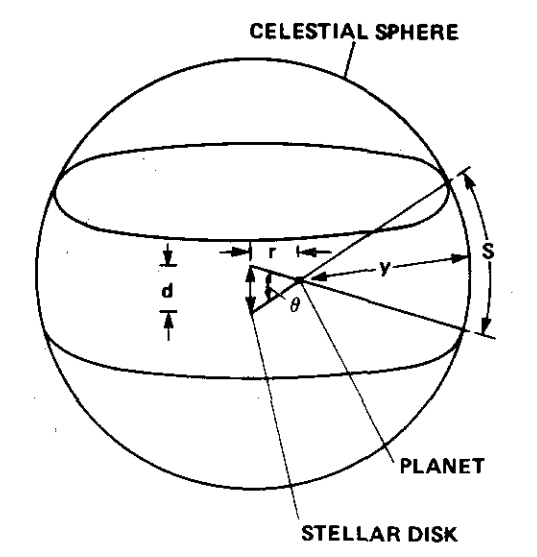
\includegraphics[width = 8cm, height = 8cm]{./Graficos/Capitulo_2/Illustrations/Prob_1.png}} 
\caption{\scriptsize{Something!}}
\label{fig:Transit_1}
\end{figure}

Now, the transit will not be produced by the point-like source but by its rings as a whole. The geometry for this scenario is shown in \autoref{fig:Transit_2} where $R_\star$ is the stellar disk radius, $a$ represents the orbital semi-major axis and $R_H$ is the Hill sphere radius. The orbital inclination of $i = 0^\circ$ means the pole is on, whilst $i = 90^\circ$ means the equator is on. The transit can occur in two different ways:\\

\begin{enumerate}
\item Grazing transit $\textnormal{a}\cos \textnormal{i} \leq \textnormal{R}_\star + \textnormal{R}_\textnormal{H}$
\item Full transit $\textnormal{a}\cos \textnormal{i} \leq \textnormal{R}_\star - \textnormal{R}_\textnormal{H}$
\end{enumerate}

\begin{figure}[!ht]
\centering
  \subfloat{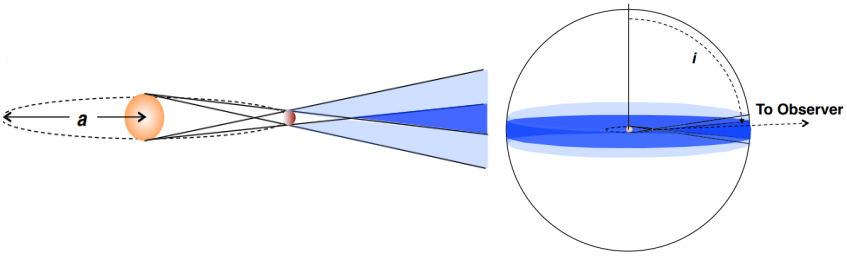
\includegraphics[width = 17cm, height = 5cm]{./Graficos/Capitulo_2/Illustrations/Prob_2.png}} 
\caption{\scriptsize{Something!}}
\label{fig:Transit_2}
\end{figure}

This is mainly dominated by the orbital inclination of the planet. Considering that the angle between the orbital inclination pole and the line of sight lies in a range ($i$, $i + \Delta i$), and it is randomly distributed as was assumed before, and also that transits occur only in nearly edge-on orbits i.e. $\textnormal{a}\cos \textnormal{i} \leq \textnormal{R}_\star + \textnormal{R}_\textnormal{H}$, we expect the probability to be uniform in $\cos \textnormal{i}$ as shown in \autoref{fig:Transit_3}. Thus, the transit probability will be given by

\begingroup
\Large
\begin{equation}
\textnormal{P} \left( \cos \textnormal{i} < \frac{\textnormal{R}_\star + \textnormal{R}_\textnormal{H}}{\textnormal{a}} \right) = \frac{\textnormal{R}_\star + \textnormal{R}_\textnormal{H}}{\textnormal{a}}
 \label{eq:ProbTransit_4}
\end{equation}
\endgroup

\begin{figure}[!ht]
\centering
  \subfloat{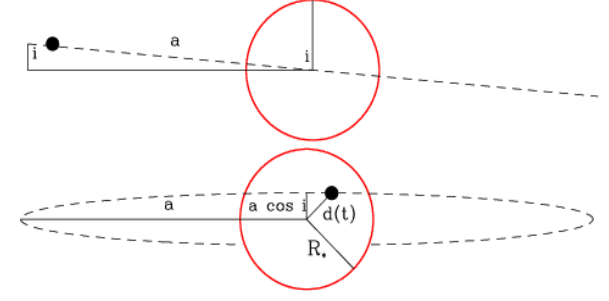
\includegraphics[width = 12cm, height = 6cm]{./Graficos/Capitulo_2/Illustrations/Prob_4.png}} 
\caption{\scriptsize{Something!}}
\label{fig:Transit_3}
\end{figure}

Then, in short, the transit probability of exoplanetary-rings in orbit around a given star where the orbital inclination is randomly distributed will be set by \autoref{eq:ProbTransit_4}, where we only need to consider the stellar and planet Hill sphere radii $R_\star$ and $R_H$ respectively, and the orbital semi-major axis. Apart from this, we need to care about when, and how long the rings can co-exist inside the Hill sphere of the planet. This probability was added at the end in order to study the overall change of what was assumed in \autoref{eq:Probabilities} and is presented in the next sub-section. 

\subsection{Rings Lifetime}\label{subsec:RingsSec}

It is well-known that the rings formation is a non-static phenomena, and there is no privileged epoch in the formation of a planetary system when these features can form. On the other hand the only example, so far, we have to compare with, is our own solar system, making the statistical comparison quite hard in terms of deriving the exact formation conditions and time ranges. Nevertheless, simulations and current observations allow us to estimate the main processes that modify these structures, and give us a glimpse on their formation timescales.\\

Currently, most of the statistics are based on \textit{Hot Jupiters} \cauthor{2013pss3.book..309T}\citeyear{2013pss3.book..309T}. However, there exists different problems with this, because the formation of rings around such objects can be affected by the low-obliquities causing the rings to edge-on or the small Hill sphere radius where they can be embedded in. In addition, viscous and Poynting-Robertson drags cause particle loss , and the high equilibrium black-body temperatures avoid materials to remain the solid state. Survival of the remnant ring depends on if they were created by tidal disruptions or continuous feeding because this will set the timescale on which the rings are expected to exist \cauthor{1984prin.conf..641H}\citeyear{1984prin.conf..641H}. In our particular case, the most important question regarding the rings is: What is their age?. This is because we need to know how long they are expected to live in order to properly compute the probability of observing ring systems around a planet given the overall age of the star and the planetary system itself. The age of the rings can be affected by the mean residence time of the particles on the rings or by how long the structure/sources have been in place For example in the case of Jupiter, if some moons suddenly disappear, or cease emitting dust, the rings will dissipate in $\sim 10^5$yr \cauthor{2013pss3.book..309T}\citeyear{2013pss3.book..309T}. Interaction and physical processes may change or reset the age as can be the shepherding of the moons inside the rings leading to an age range of $100\times 10^6$-$6\times10^8$yr \cauthor{1994P&SS...42.1139C}\citeyear{1994P&SS...42.1139C}, or ring's viscous spreading ($10^5$-$10^9$yr based on Saturn's ring A) \cauthor{2009sfch.book..537C}\citeyear{2009sfch.book..537C} or ($\sim10^9$yr) from viscous timescales if the gas is considered to be non-turbulent \cauthor{1984prin.conf..641H}\citeyear{1984prin.conf..641H}. There exists also the chance that the ring is completely disrupted (based on the fragmentation criteria), so in that case we end up with a time for complete loss of the rings of $10^{7}$-$10^8$yr \cauthor{1994P&SS...42.1139C}\citeyear{1994P&SS...42.1139C} or based on evolutionary processes $< 10^8$yr \cauthor{2009sfch.book..537C}\citeyear{2009sfch.book..537C}. On the other hand, considering cometary passages which could break a satellite or to tidally disrupt the comet applied to Saturn's ring lead to a time range of $10^7$-$10^8$yr for the A-ring, $10^8$-$10^9$yr for the B-ring, and $10^7$yr from radial spreading \cauthor{2009sfch.book..537C}\citeyear{2009sfch.book..537C}.\\

As has been presented above, different age ranges can be derived for the rings lifetime through models and observations of our own solar system. However, the remaining question is: Do they form at the very beginning, the middle or the end of the planetary system formation?. According to \cauthor{2009Icar..199..413C}\citeyear{2009Icar..199..413C} the main core of Saturn's B-ring was formed in the first Gyr of the solar system in which collisions are expected to be much more likely. However, from simulations it is pointed out Saturn's ring formation can be understood a huge disruption near the end of the planetary formation period during which the circum-planetary gas disk is still present \cauthor{2010Natur.468..943C}\citeyear{2010Natur.468..943C}. If we look to Uranus or Neptune, possibly they have been less affected and have not changed dramatically over the age of the solar system, where rings and moons has been oscillating between accretion and disruption for many Gyr \cauthor{2013pss3.book..309T}\citeyear{2013pss3.book..309T}.\\

In general, there is no complete consensus on whether the rings form at the beginning, or at the end of the planetary formation process, neither on the time they can live as a ring-structure around the planet. Base don this, we decided to introduce a fifth probability to account for the most likely lifespan a ring can have. The probability is defined in \autoref{eq:Prob_5}, but it is necessary to have in mind that as it is hard to guarantee the exact moment in time where they form, then this probability assumes each time interval has the same chance and we can only provide an estimation based on the mean-rings lifespan and the stellar age.  

\begingroup
\Large
\begin{equation}
\textnormal{P}_5 = \frac{\textnormal{Rings}~\textnormal{lifespan}}{\textnormal{Host}~\textnormal{star's}~\textnormal{age}}
 \label{eq:Prob_5}
\end{equation}
\endgroup

%============================================================================================================================================================

\section{Monte-Carlo simulations}\label{sec:MCSec}

\begin{figure}[!ht]
\centering
  \subfloat{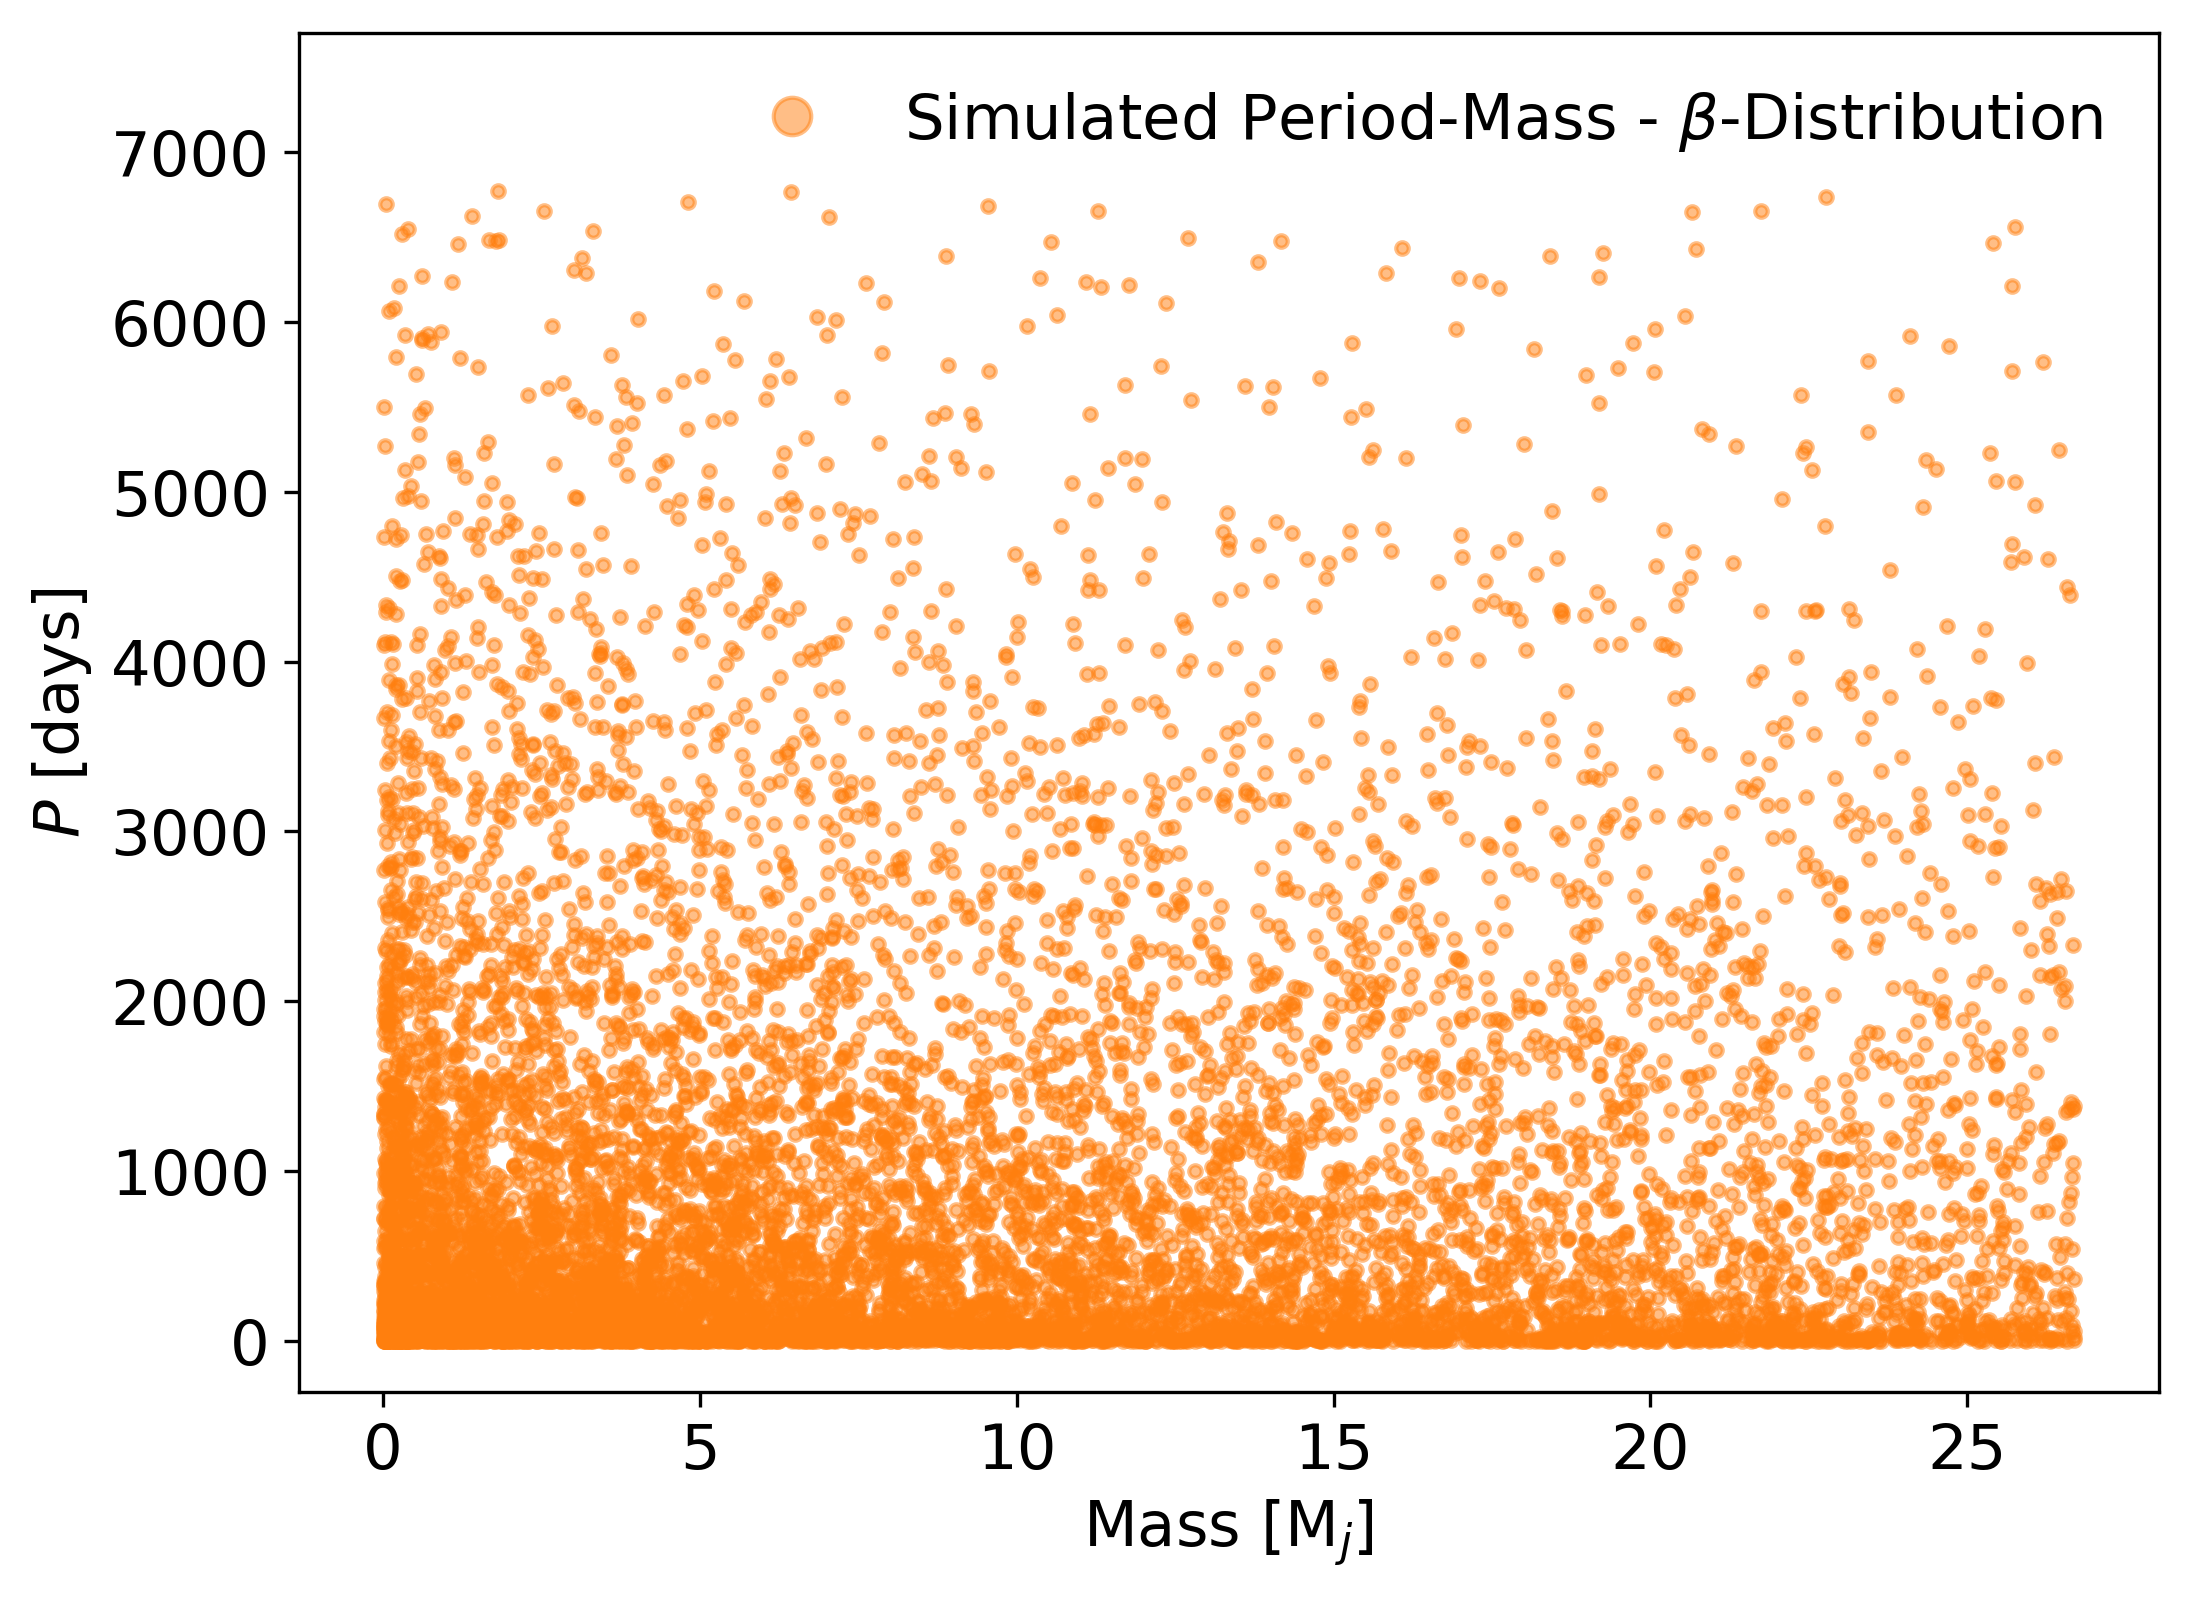
\includegraphics[width = 12cm, height = 9cm]{./Graficos/Capitulo_2/2_Exop_distributions/Period_mass_distribution_2.png}} 
\caption{\scriptsize{Something!}}
\label{fig:PeriodMass_Beta}
\end{figure}

\begin{figure}[!ht]
\centering
  \subfloat{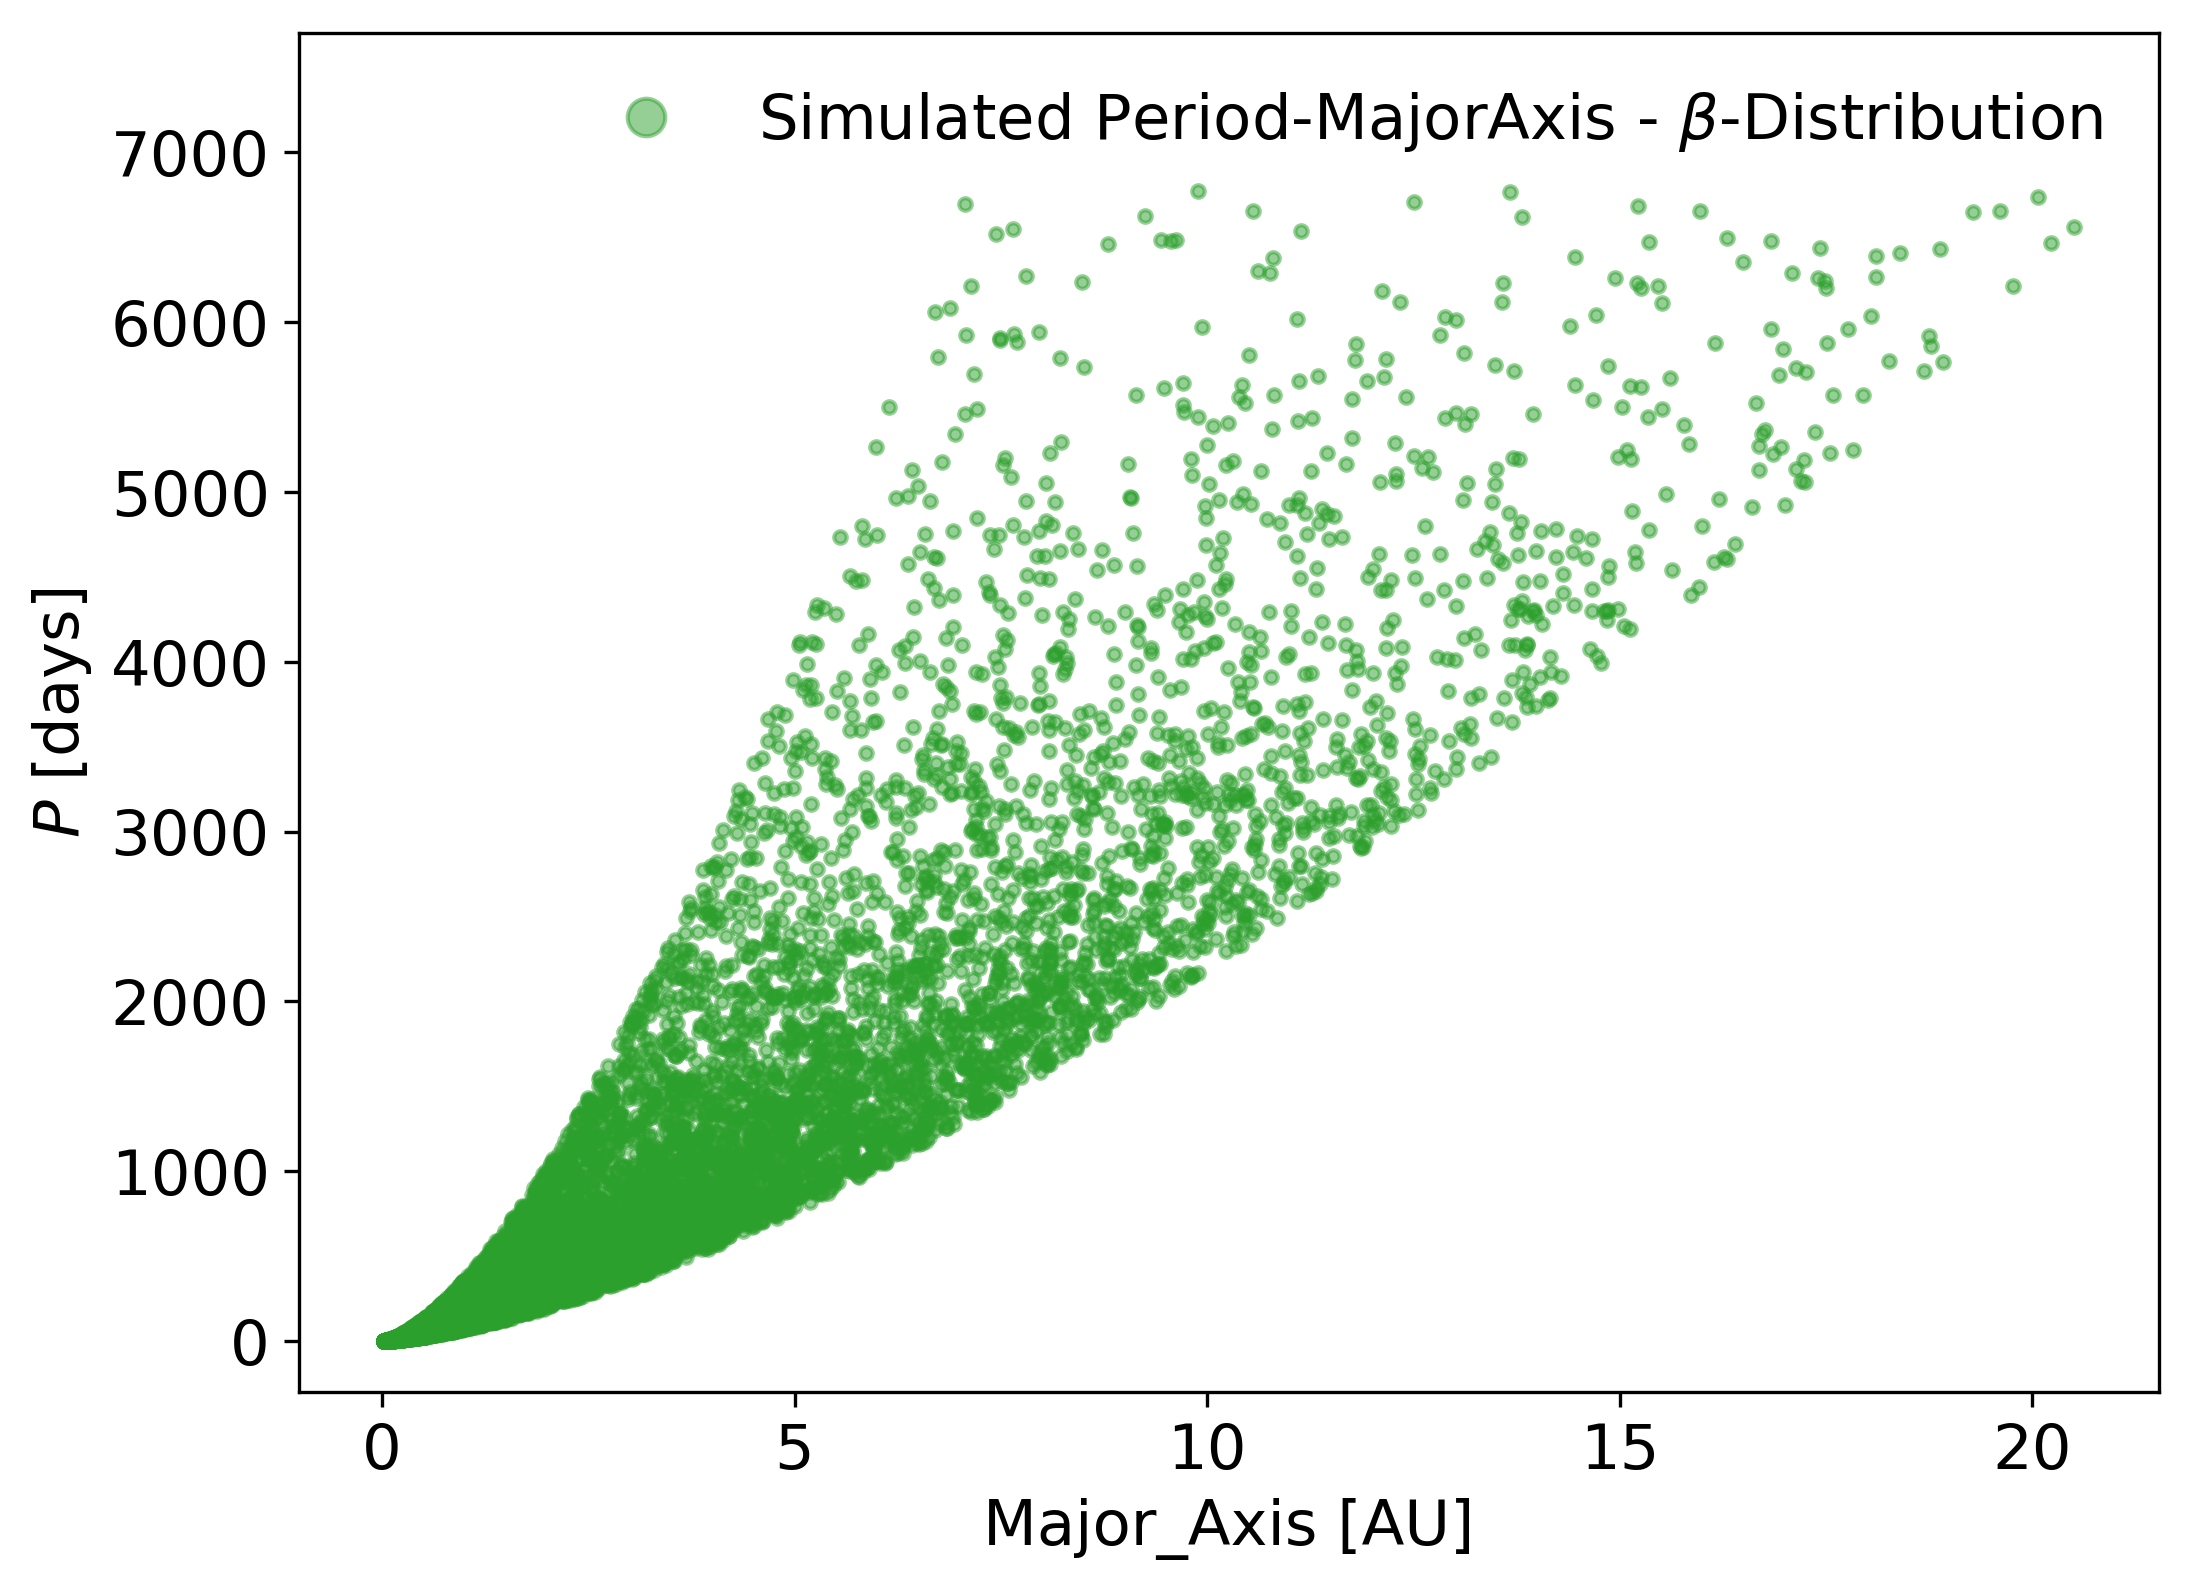
\includegraphics[width = 12cm, height = 9cm]{./Graficos/Capitulo_2/2_Exop_distributions/Period_major_distribution_2.png}} 
\caption{\scriptsize{Something!}}
\label{fig:PeriodMajor_Beta}
\end{figure}

\begin{figure}[!ht]
\centering
  \subfloat{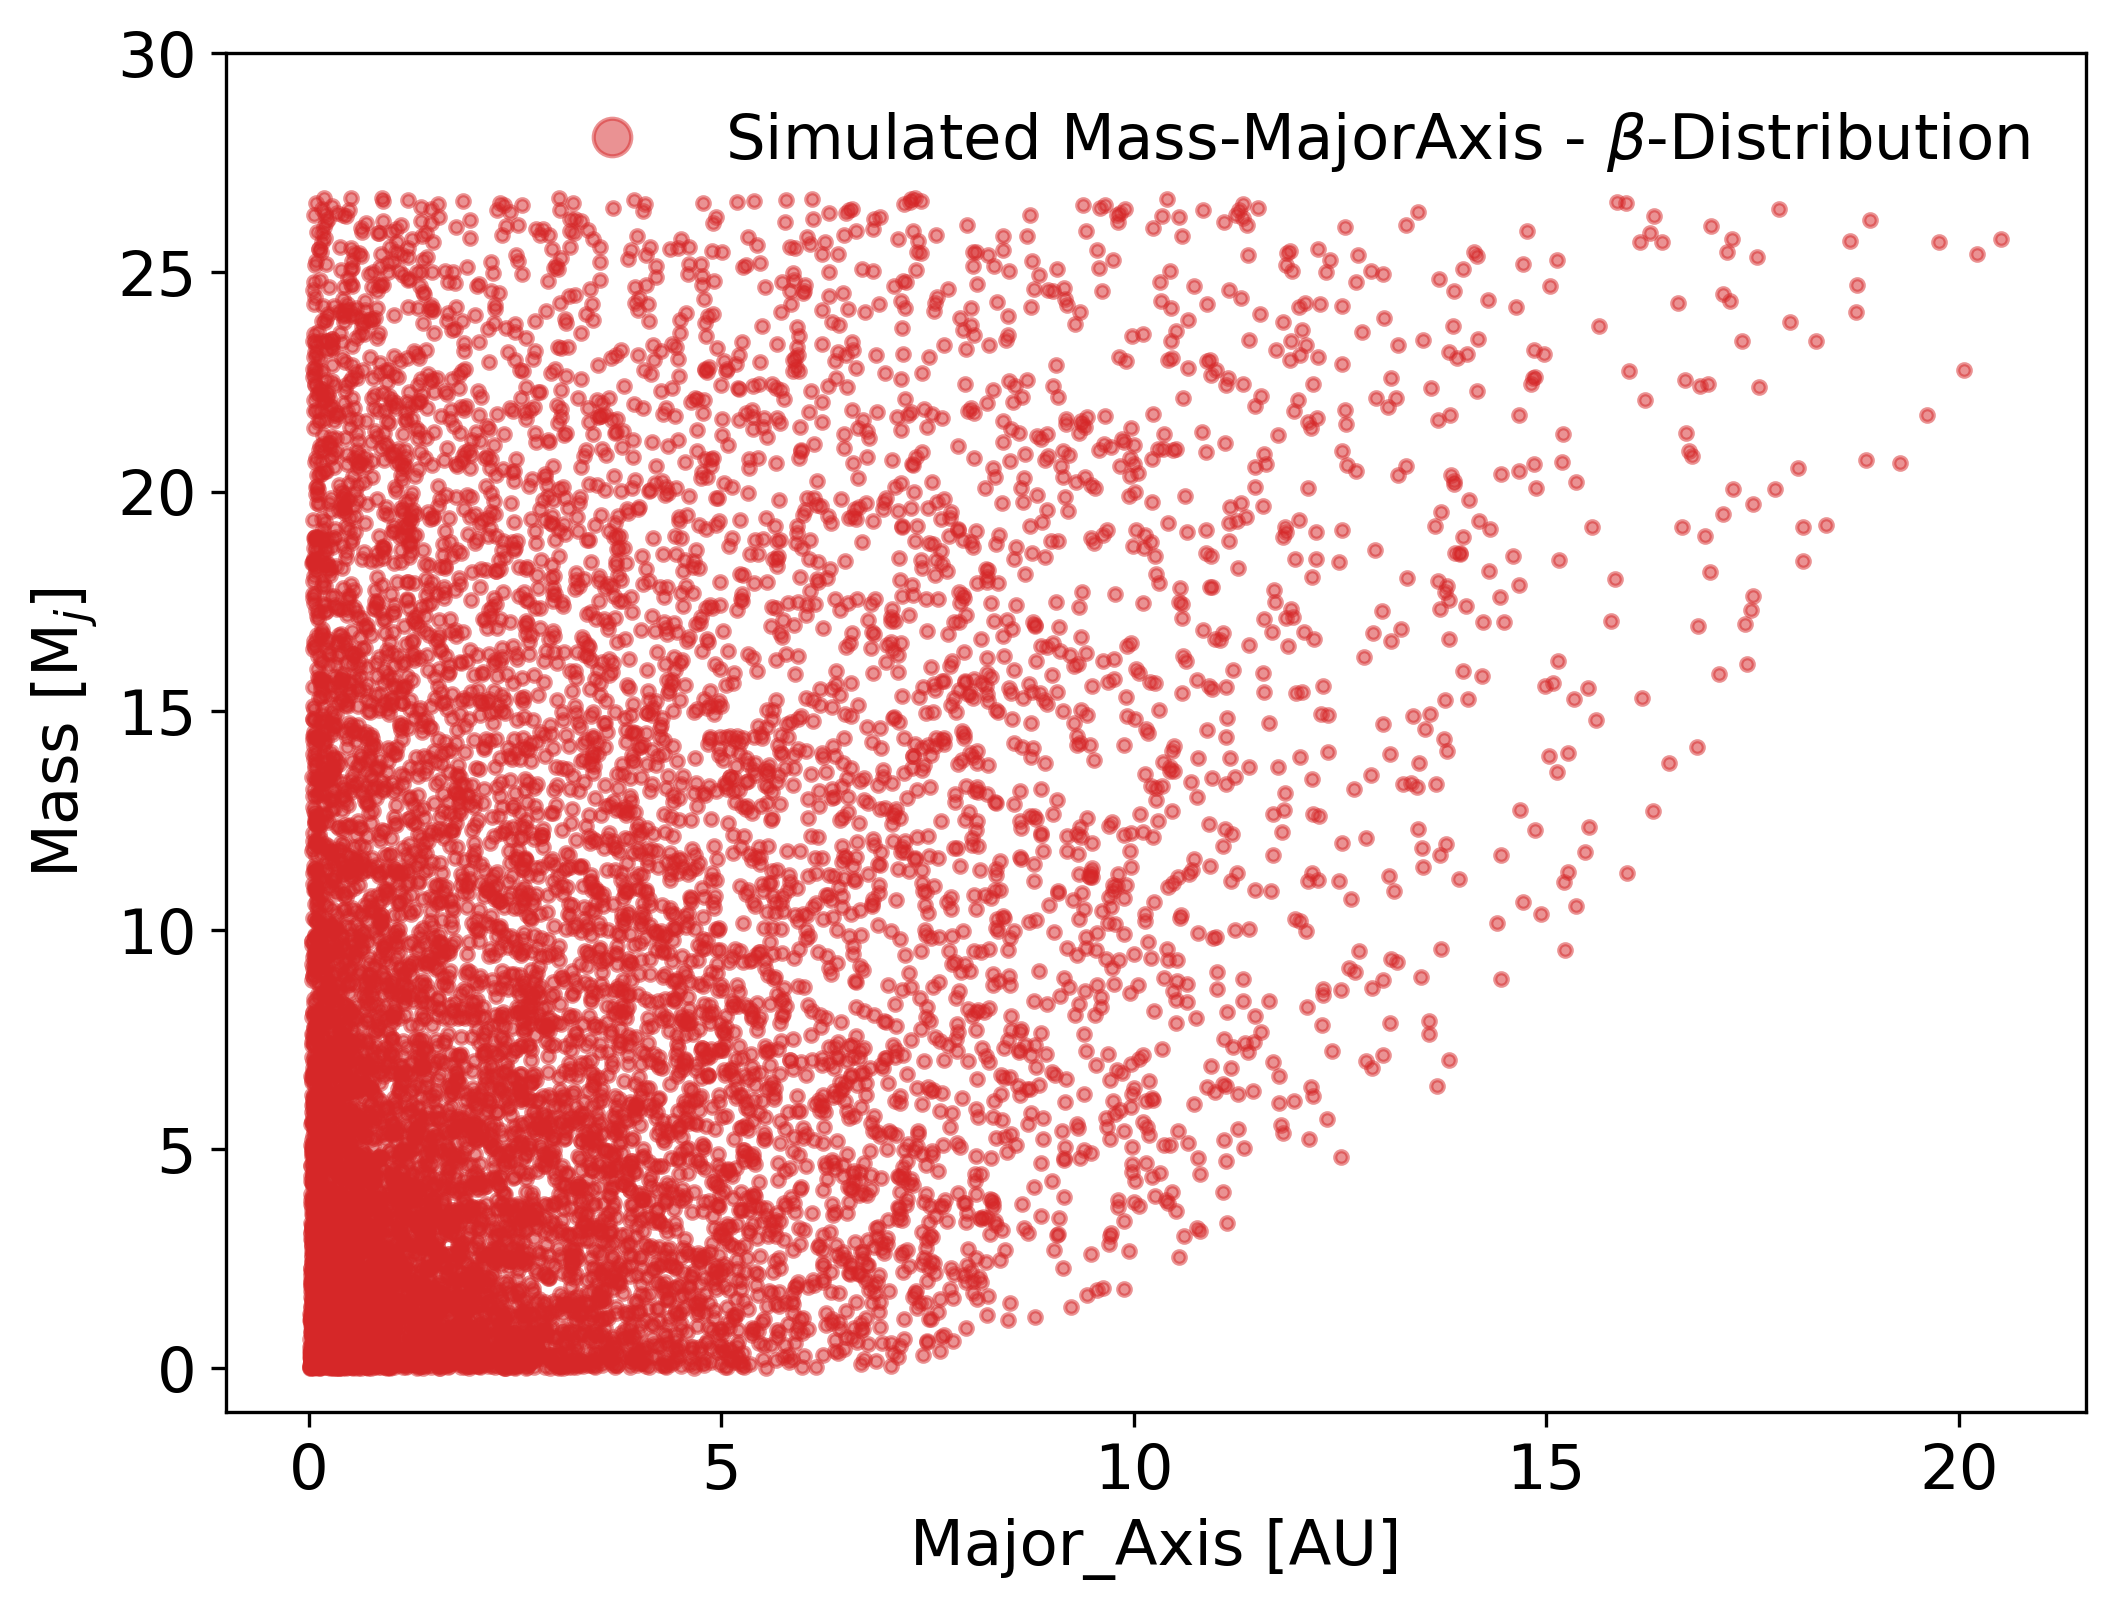
\includegraphics[width = 12cm, height = 9cm]{./Graficos/Capitulo_2/2_Exop_distributions/Mass_major_distribution_2.png}} 
\caption{\scriptsize{Something!}}
\label{fig:MassMajor_Beta}
\end{figure}

\begin{figure}[!ht]
\centering
  \subfloat{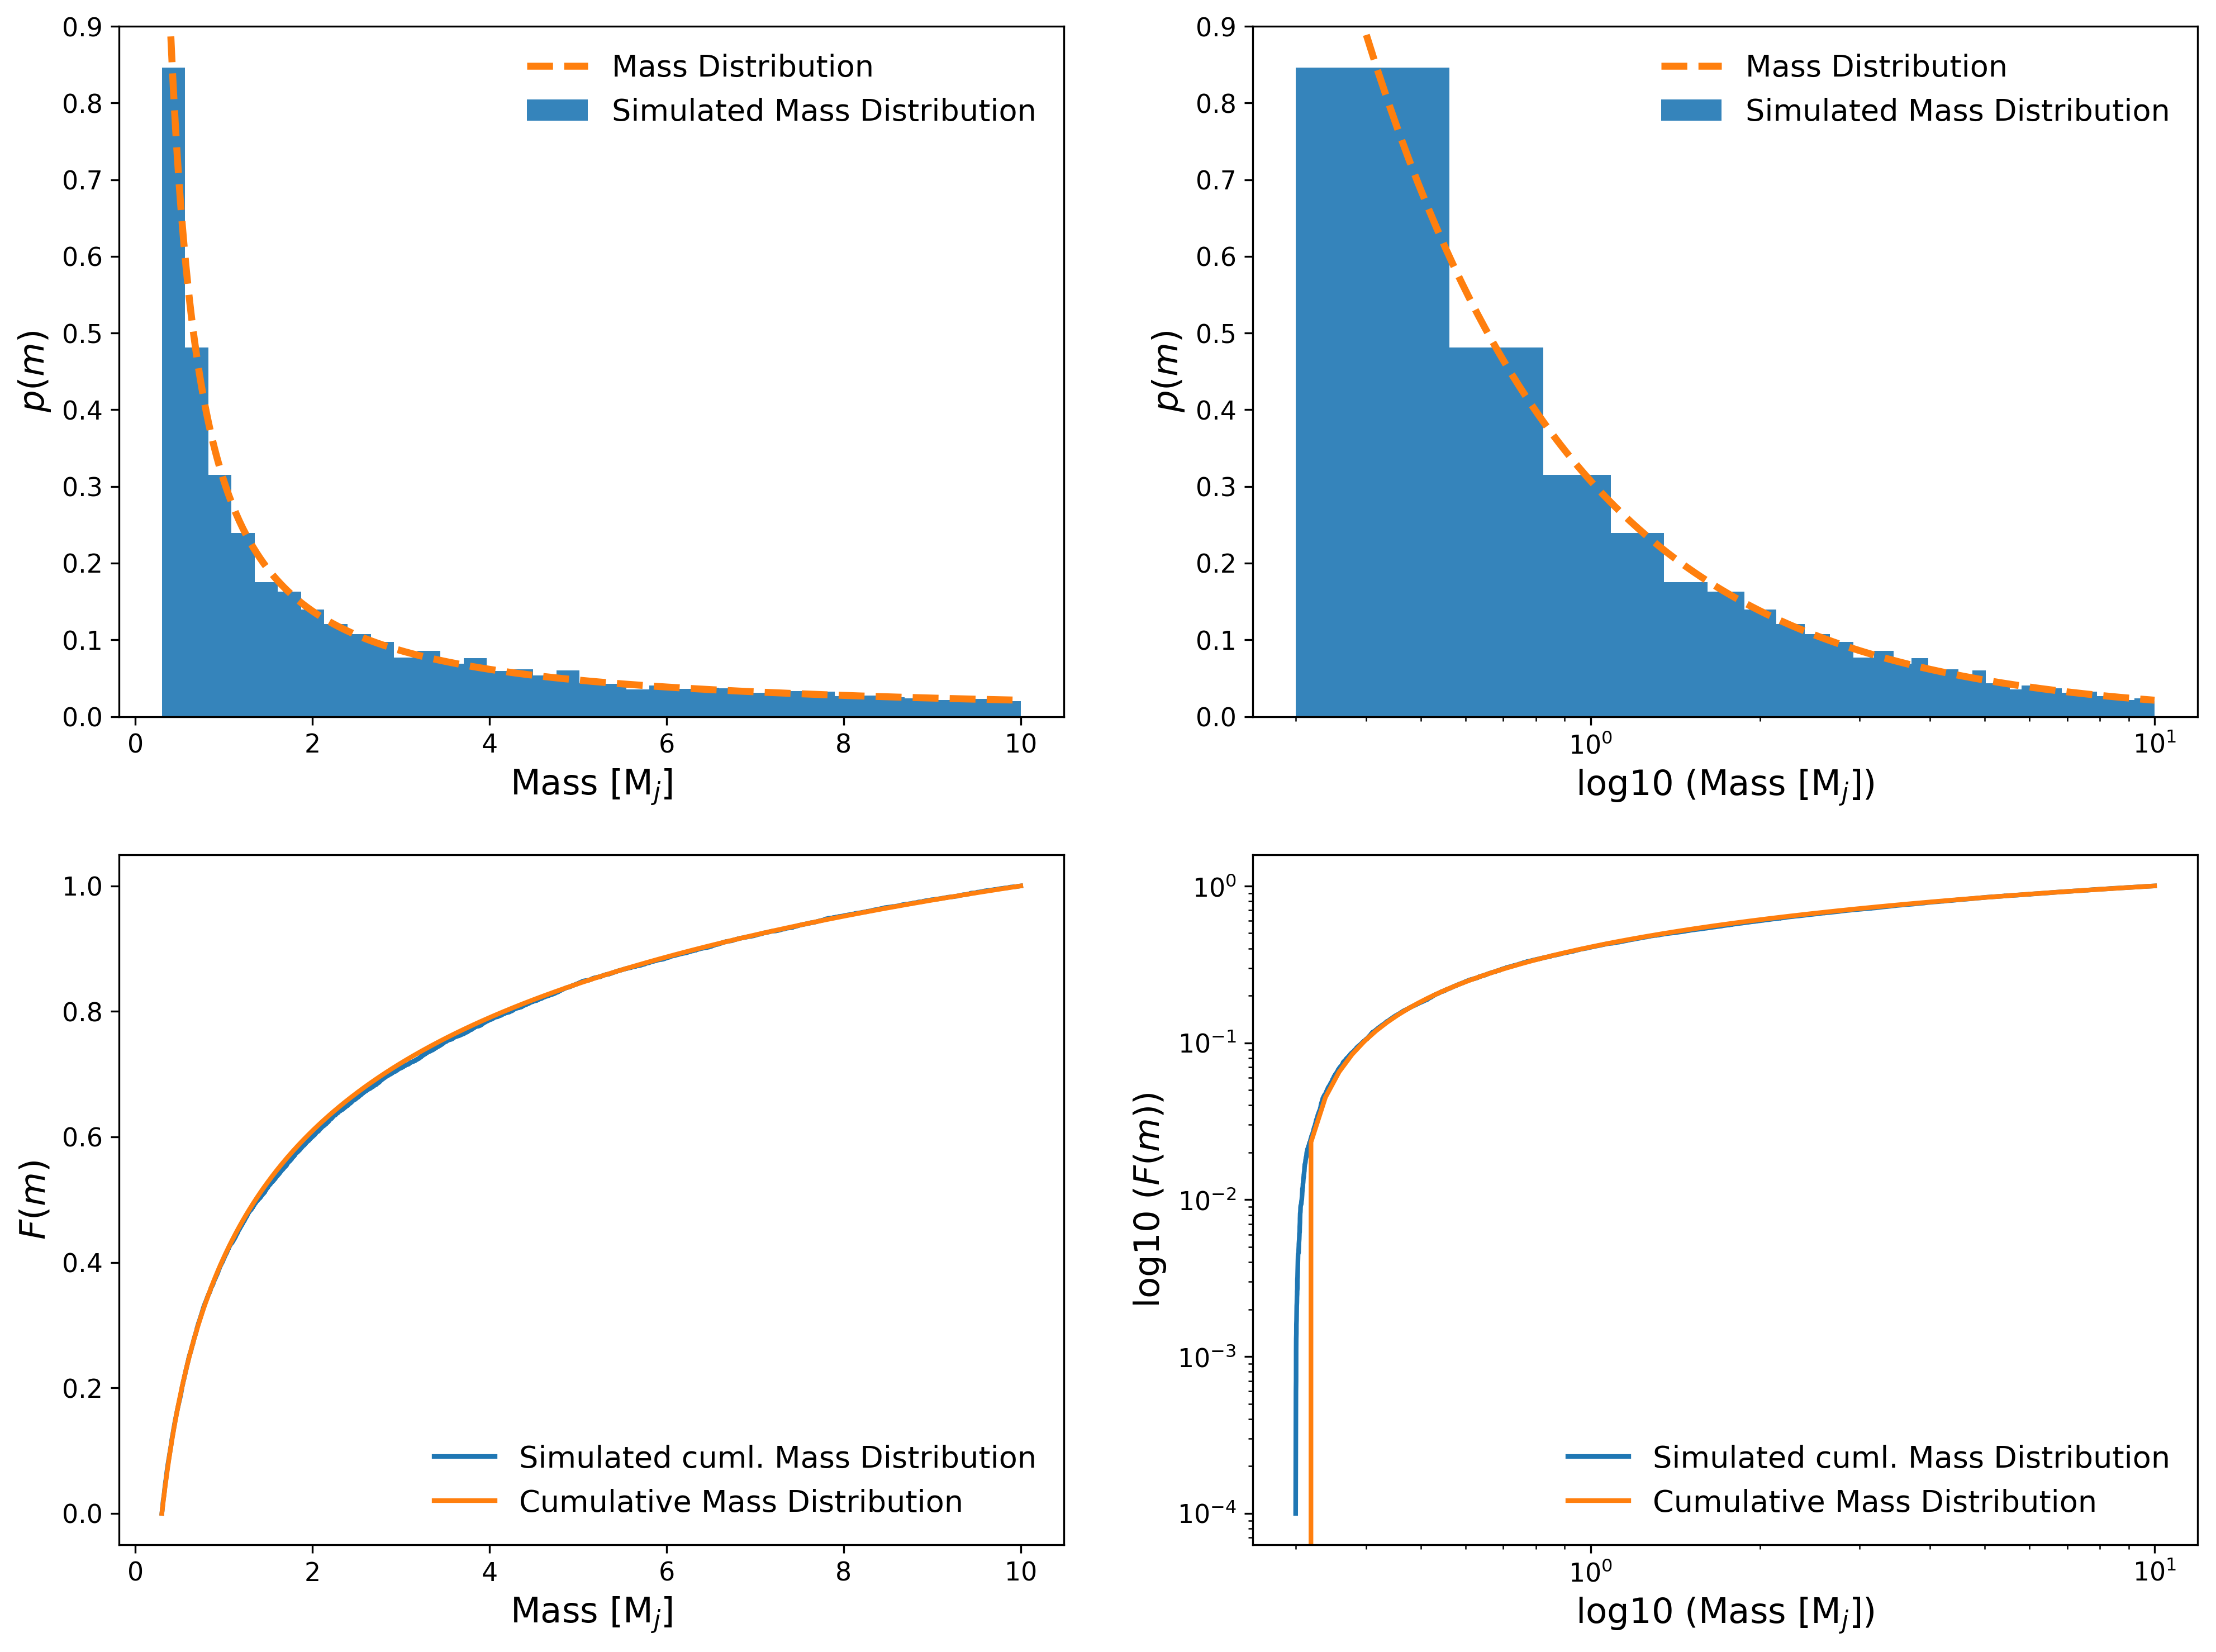
\includegraphics[width = 18.5cm, height = 15.5cm, scale = 1.0, angle = 90]{./Graficos/Capitulo_2/2_Exop_distributions/Mass_distribution_Nielsen.png}} 
\caption{\scriptsize{Something!}}
\label{fig:Mass_Nielsen}
\end{figure}

\begin{figure}[!ht]
\centering
  \subfloat{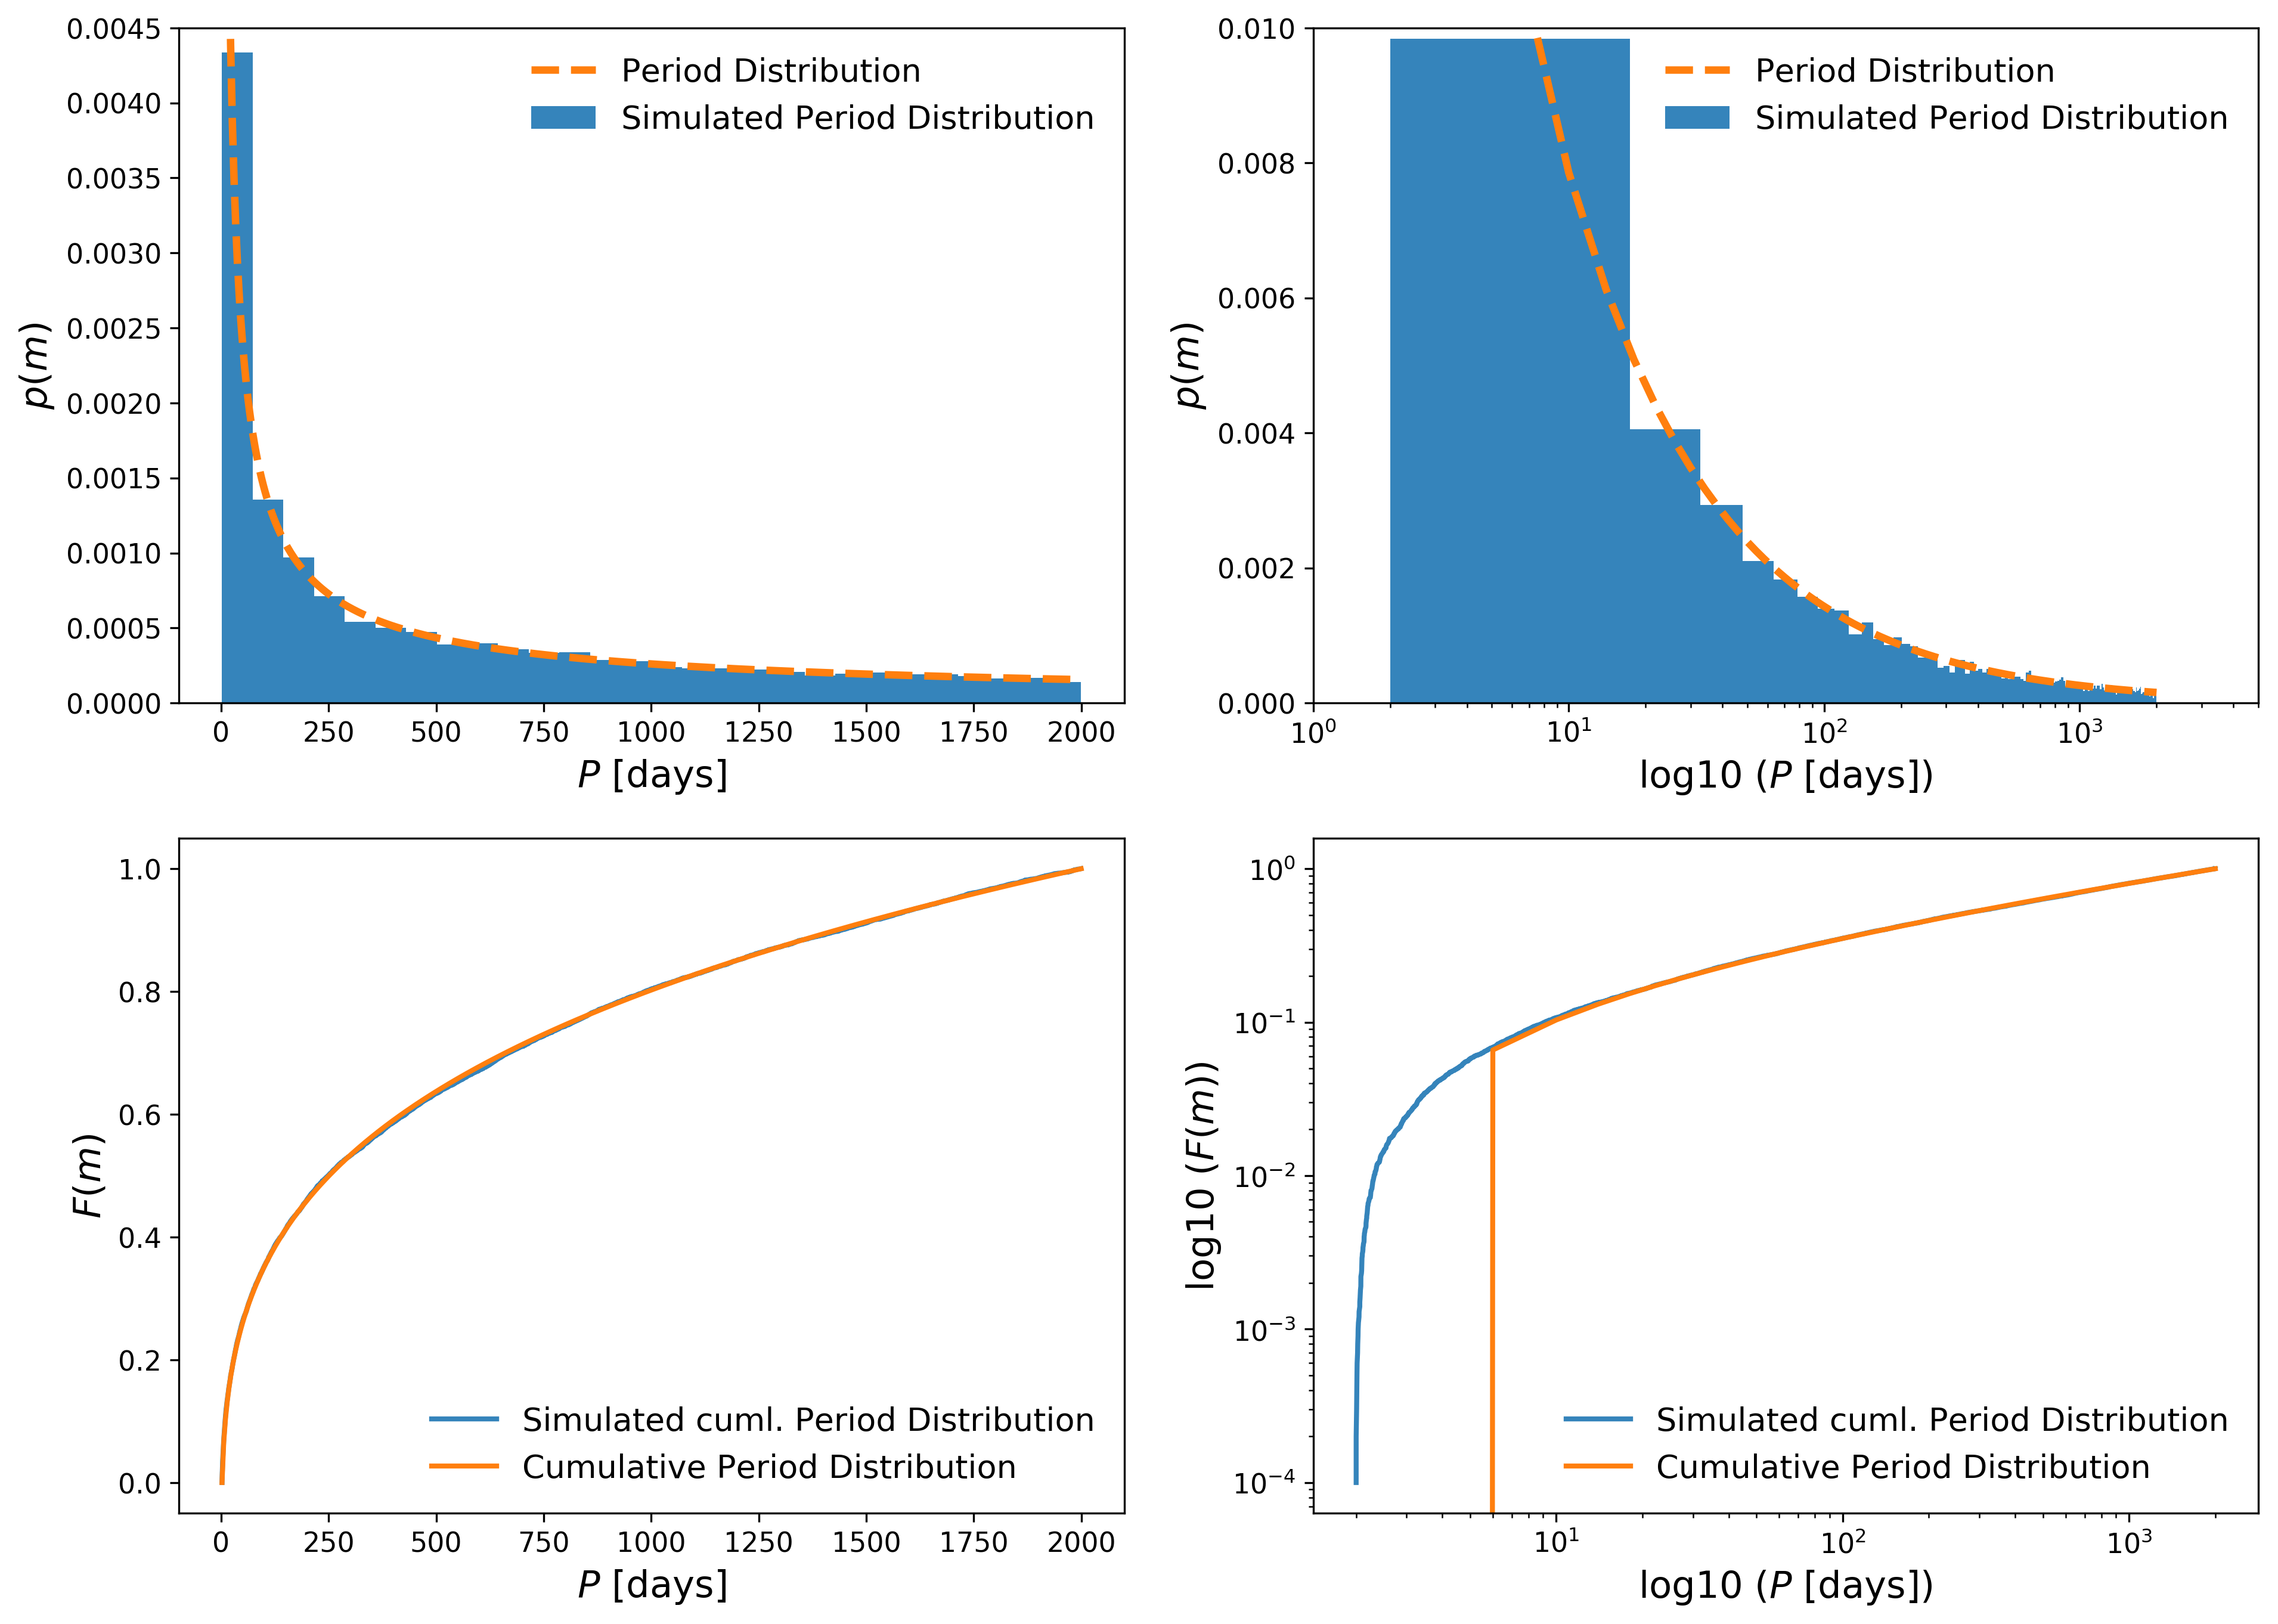
\includegraphics[width = 18.5cm, height = 15.5cm, scale = 1.0, angle = 90]{./Graficos/Capitulo_2/2_Exop_distributions/Period_distribution_Nielsen.png}} 
\caption{\scriptsize{Something!}}
\label{fig:Mass_Nielsen}
\end{figure}

\begin{figure}[!ht]
\centering
  \subfloat{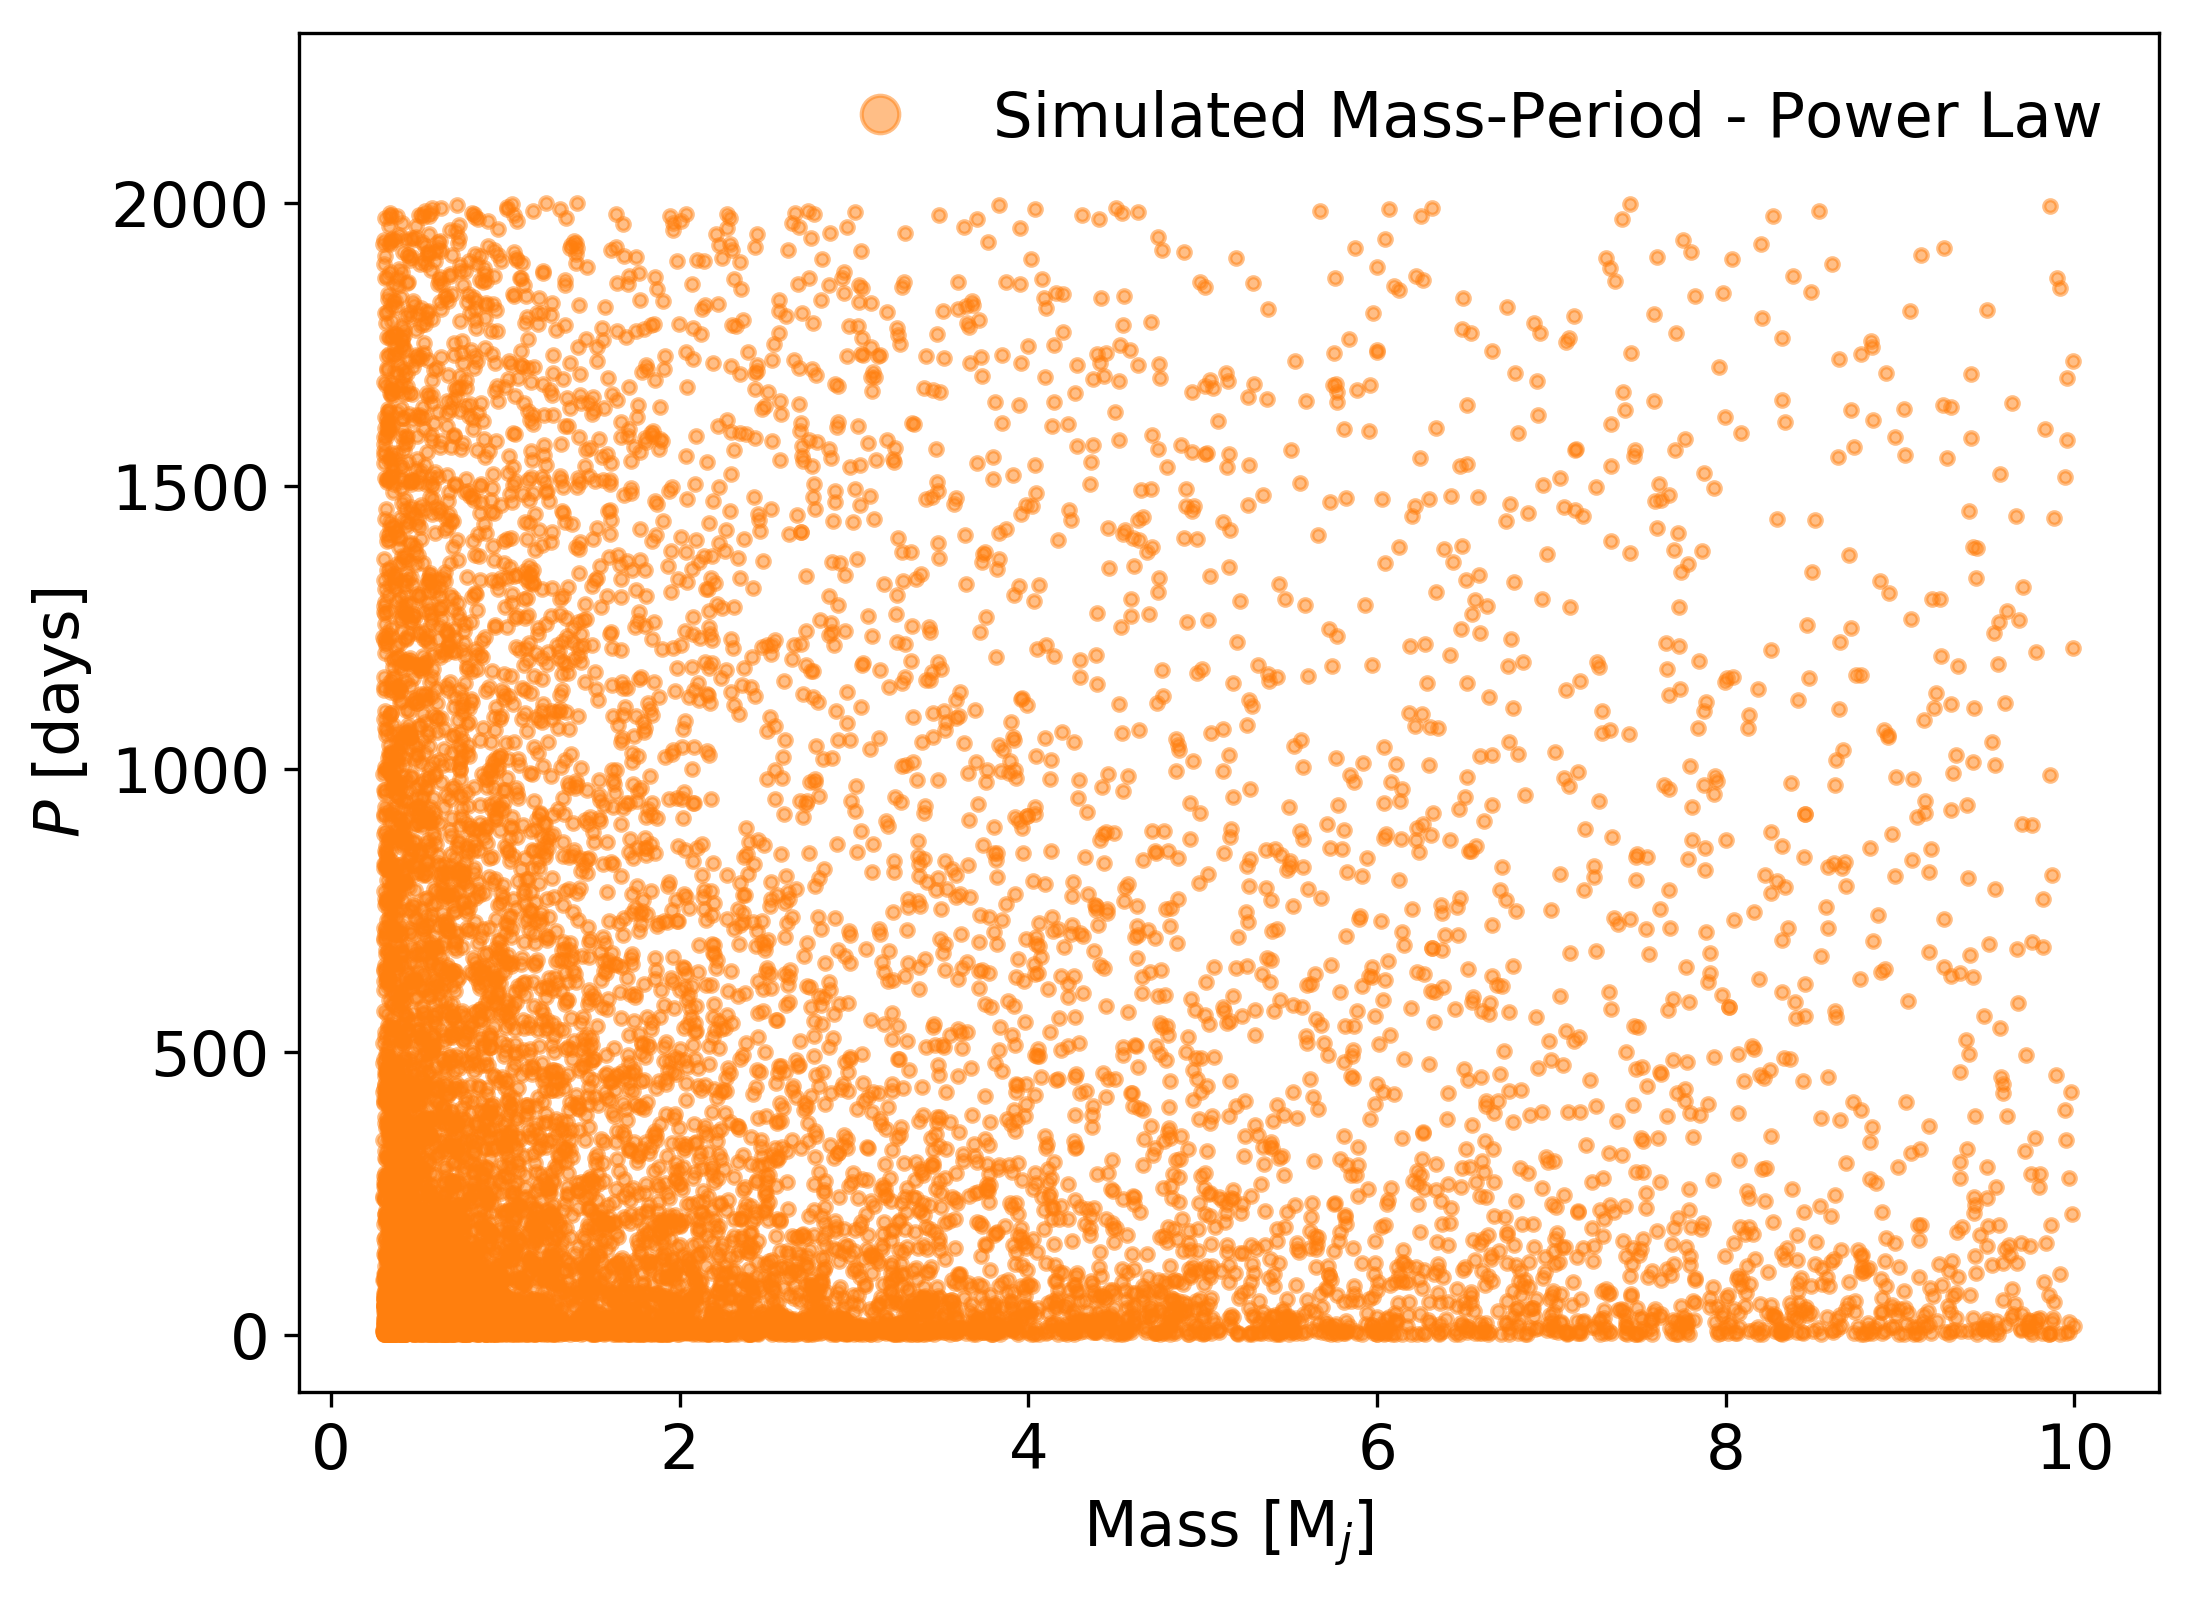
\includegraphics[width = 12cm, height = 9cm]{./Graficos/Capitulo_2/2_Exop_distributions/Period_mass_distribution.png}} 
\caption{\scriptsize{Something!}}
\label{fig:PeriodMass_Nielsen}
\end{figure}

\begin{figure}[!ht]
\centering
  \subfloat{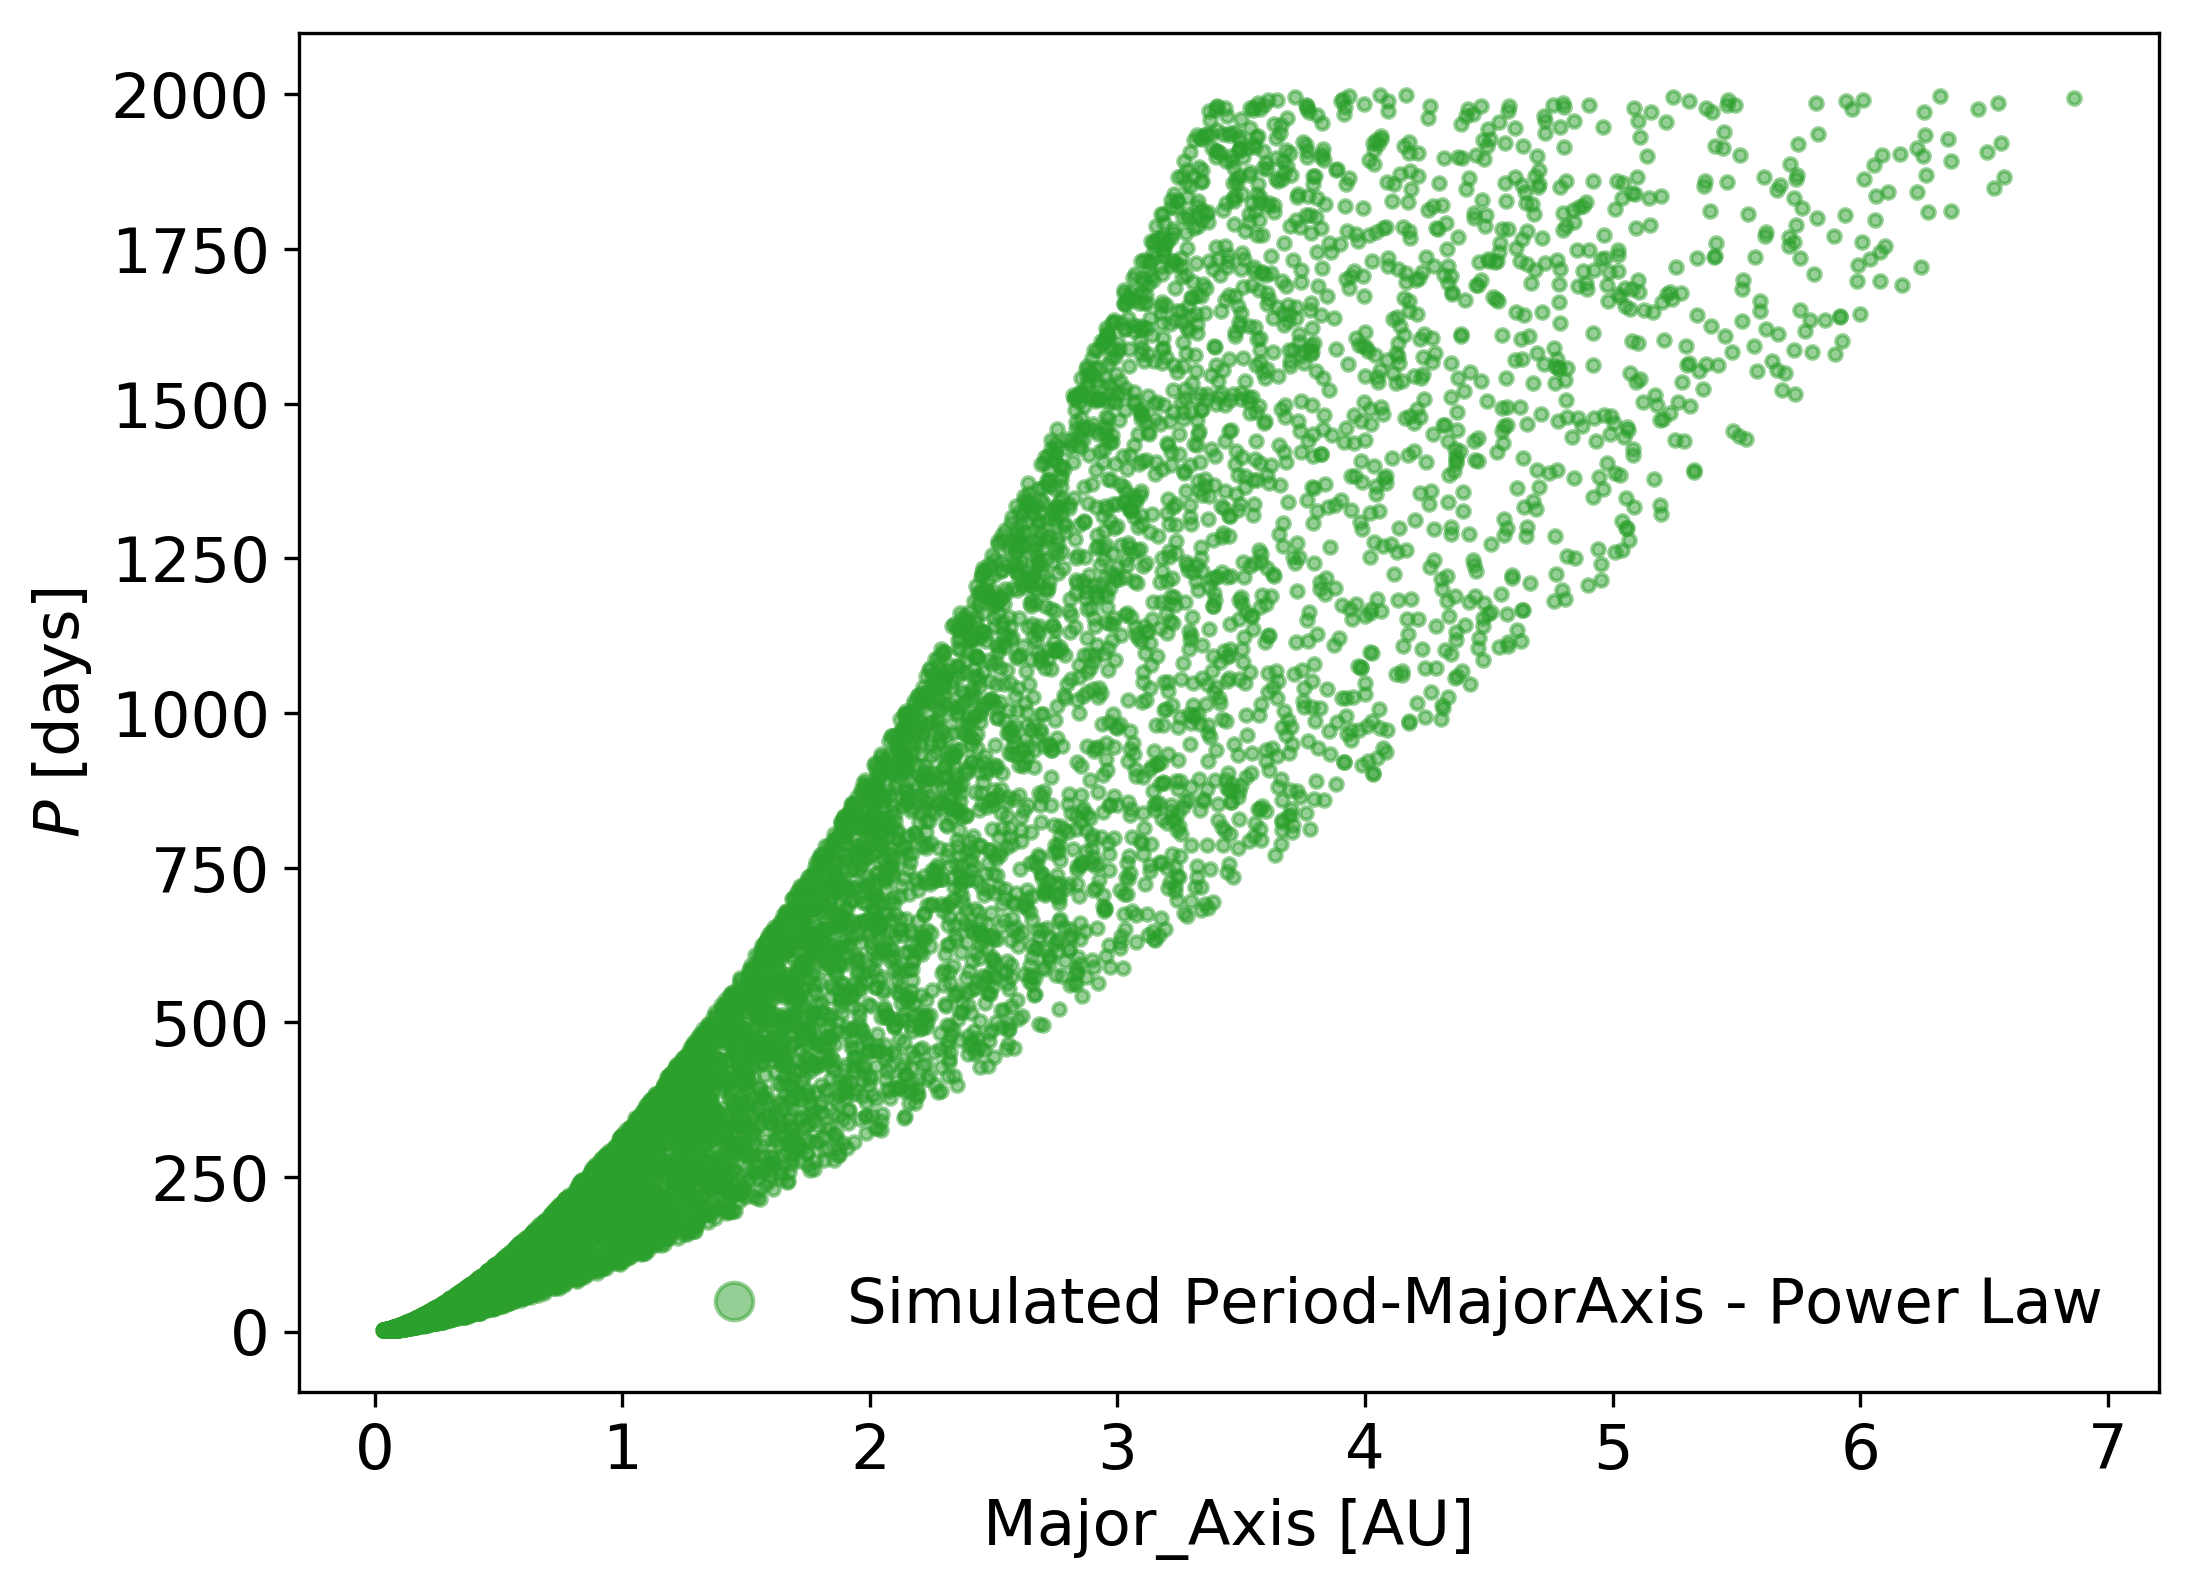
\includegraphics[width = 12cm, height = 9cm]{./Graficos/Capitulo_2/2_Exop_distributions/Period_major_distribution.png}} 
\caption{\scriptsize{Something!}}
\label{fig:PeriodMajor_Nielsen}
\end{figure}

\begin{figure}[!ht]
\centering
  \subfloat{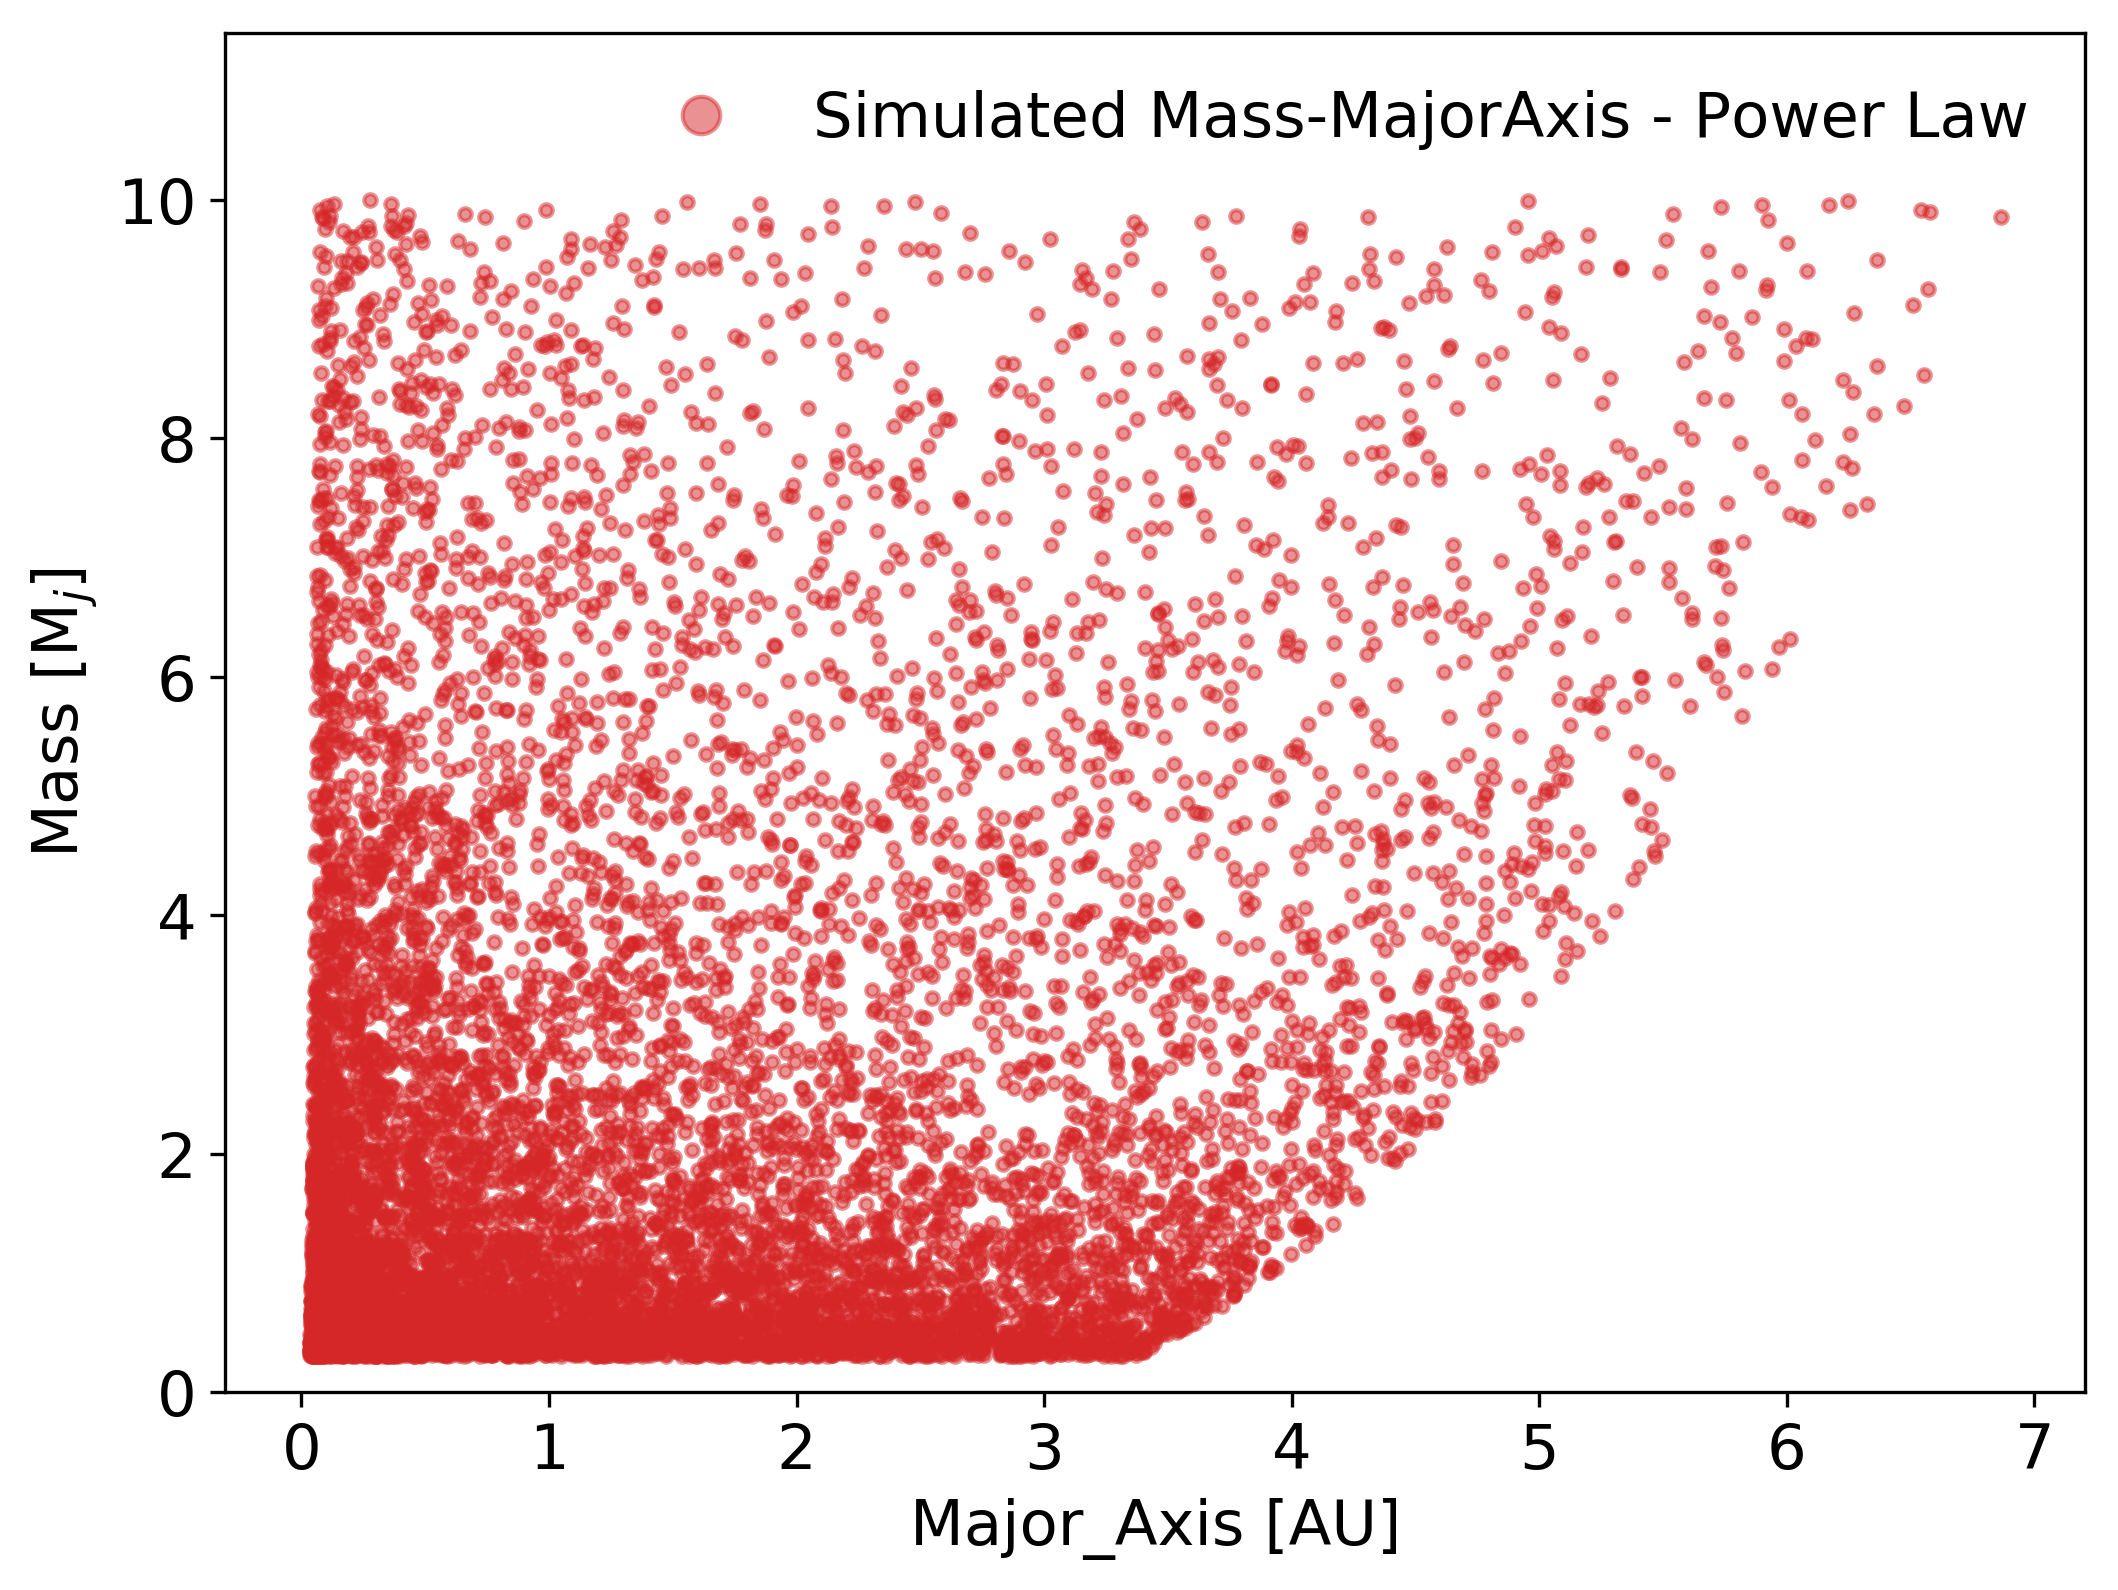
\includegraphics[width = 12cm, height = 9cm]{./Graficos/Capitulo_2/2_Exop_distributions/Mass_major_distribution.png}} 
\caption{\scriptsize{Something!}}
\label{fig:MassMajor_Nielsen}
\end{figure}


%============================================================================================================================================================

\section{Analytic Form}
%============================================================================================================================================================
